% TODO specify all measures as complex
% TODO make everythin Hausdorff???
% TODO laga kápu
% TODO make sure at the end that 'Caratheodory' is nowhere
% TODO fix open intervals. they look ugly
% TODO decide if 0 is in \mathbb{N} and make sure it's consistent
% TODO read and mention Globevnik
% TODO in F. and M. Riesz chapter talk about why the function spaces are seperable
\documentclass[a4paper,12pt,twoside,BCOR=10mm]{scrbook}

% Packages
\usepackage{ucs}
\usepackage[utf8x]{inputenc}
\usepackage[icelandic, english]{babel}
\usepackage{t1enc}
\usepackage{graphicx}
\usepackage[intoc]{nomencl}
\usepackage{enumerate,color}
\usepackage{url}
\usepackage[pdfborder={0 0 0}]{hyperref}
\usepackage{appendix}
\usepackage{eso-pic}
\usepackage{amsmath}
\usepackage{amsthm}
\usepackage{amssymb}
\usepackage[nottoc]{tocbibind}
\usepackage[sort&compress,authoryear]{natbib}
\bibliographystyle{plainnat}
\usepackage[sf,normalsize]{subfigure}
\usepackage[format=plain,labelformat=simple,labelsep=colon]{caption}
\usepackage{placeins}
\usepackage{tabularx}
\usepackage{mathabx}
\usepackage{mathtools}
\usepackage{wrapfig}
% Configurations
\graphicspath{{figs/}}

\newtheorem{theorem}{Theorem}[section]
\newtheorem{corollary}[theorem]{Corollary}
\theoremstyle{definition}
\newtheorem{remark}[theorem]{Remark}
\theoremstyle{definition}
\newtheorem{example}{Example}
\newtheorem{lemma}[theorem]{Lemma}
\theoremstyle{definition}
\newtheorem{definition}[theorem]{Definition}
\renewcommand{\Re}{\text{Re }}
\renewcommand{\Im}{\text{Im }}

\setlength{\parskip}{\baselineskip}
\setlength{\parindent}{0cm}
\raggedbottom
% \setkomafont{subsection}{\normalfont\sffamily}

% Eins og templatið á að vera
% \setkomafont{captionlabel}{\itshape}
% \setkomafont{caption}{\itshape}

% Mun fallegri lausn
\setkomafont{captionlabel}{\itshape}
\setkomafont{caption}{\itshape}
\setkomafont{section}{\FloatBarrier\Large}
\setcapwidth[l]{\textwidth}
\setcapindent{1em}


% Times new roman
%\usepackage[T1]{fontenc}
%\usepackage{mathptmx}

%%%%%%%%%%% MODIFY THESE LINES ONLY %%%%%%%%%%%%%%%%%%%%%%%%%%%%%%%%%%%%%%%%%%%%%%%%%%%%%%%%%
\def\thesisyear{2020}       						% Year thesis submitted
\def\thesismonth{XXmonth}						% Month thesis submitted
\def\thesisauthor{Bergur Snorrason}					% Thesis authoreiningaraðferðinni
\def\thesistitle{XXTitle} 						% Title of thesis
\def\thesisshorttitle{XXShort title (50 characters including spaces)} 	% Title of thesis
\def\thesiscredits{XX} 							% Credits awarded for the project
\def\thesissubject{XX}
\def\thesiskind{M.Sc.}							% Masters of PhD thesis
\def\thesiskindformal{Magister Scientiarum}				% Masters of PhD thesis
\def\thesisnroftutors{1}						% Number of tutors
\def\thesisschool{School of Engineering and {Natural Sciences}}		% School
\def\thesisfaculty{XX}							% Faculty
\def\thesisaddress{XXFaculty street address}				% Office address
\def\thesispostalcode{XXFaculty postal code, Reykjavik}			% Office address
\def\thesistelephone{525 4000}						% Office telephone
\def\thesispublisher{XX}						% Publisher
\def\thesistutors{XXNN1 \\ XXNN2}
\def\thesisrepresentative{XXNN3}					% Tutors name
\def\thesiscommittee{XXNN4 \\ XXNN5 }
\def\thesiskeywords{Keyword1, Keyword2, Keyword3}			% Keywords
\def\thesisISBN{XX}           						% Thesis ISBN number
\def\thesisdedication{Dedication}
\def\thesisPrinting{Háskólaprent, Fálkagata 2, 107 Reykjavík}

% Function to add footer to frontpage
\newcommand\BackgroundPic{
\put(0,0){
\parbox[b][\paperheight]{\paperwidth}{
\vfill
\centering
\hspace*{-0.6cm}

\includegraphics[width=\paperwidth,height=\paperheight,
keepaspectratio]{foot}
}}
\setlength{\unitlength}{\paperwidth}
\begin{picture}(0,0)(0,-0.15)
\put(0,0){\color{white}\parbox{1\paperwidth}{\centering\bfseries\sffamily \Large Faculty of \thesisfaculty \\
University of Iceland\\
\thesisyear}}
\end{picture}
}

\begin{document}

\begin{titlepage}
\thispagestyle{empty}
\AddToShipoutPicture*{\BackgroundPic}
%
\begin{center}
\vspace*{1cm}

\includegraphics[width=43.6mm]{ui_1_cmyk}\\
\vspace*{3.0cm}
\huge \sffamily \bfseries \thesistitle

\vspace*{5.5cm}
\normalfont \Large \sffamily \thesisauthor
\AddToShipoutPicture*{\BackgroundPic}
\vfill

\end{center}

\newpage 
\thispagestyle{empty} \mbox{}
\newpage
\vspace*{1.35cm}
\thispagestyle{empty}
\begin{center}

\Large \textbf{\sffamily{\MakeUppercase{\thesistitle}}} \\

\vspace*{1.7cm}
\sffamily{\thesisauthor} \\
\vspace*{1.8cm}
\normalsize \thesiscredits~ECTS thesis submitted in partial fulfillment of a \\
\textit{\thesiskindformal} degree in \thesissubject

\vspace*{1.0cm}
\large
\ifnum\thesisnroftutors >1 Advisors \\ \thesistutors \\ \vspace*{0.4cm}
\else Advisor \\ \thesistutors \\ \vspace*{1.04cm}
\fi
Faculty Representative \\
\thesisrepresentative

\vspace*{0.4cm}
M.Sc. committee \\
\thesiscommittee

\vfill
Faculty of \thesisfaculty \\
\thesisschool \\
University of Iceland \\
Reykjavik, \thesismonth~\thesisyear
\newpage
\end{center}
 \newpage
 \thispagestyle{empty}
 \mbox{} \vfill
 % \setcounter{page}{0} \renewcommand{\baselinestretch}{1.5}\normalsize
 \sffamily{\thesistitle} \\
 \sffamily{\thesisshorttitle} \\
 \thesiscredits ~ECTS thesis submitted in partial fulfillment of a \thesiskind~degree in \thesissubject
\\ \\
Copyright \textcopyright~\thesisyear~ \thesisauthor \\
All rights reserved \\


Faculty of \thesisfaculty \\
\thesisschool \\
University of Iceland \\
\thesisaddress \\
\thesispostalcode, Reykjavik \\
Iceland

Telephone: \thesistelephone \\ \\
\vspace*{\lineskip}

Bibliographic information: \\
\thesisauthor, \thesisyear, \thesistitle, \thesiskind~thesis, Faculty of \thesisfaculty, University of Iceland. \\

ISBN~\thesisISBN

Printing: \thesisPrinting \\
Reykjavik, Iceland, \thesismonth~\thesisyear \\
\newpage
\thispagestyle{empty} \mbox{}
\vfill
\begin{center}\textit{\thesisdedication}\end{center} \vspace*{5cm}
\vfill 

\thispagestyle{empty}
\cleardoublepage
\end{titlepage}


% \dedication{\textit{Dedication} \small \\ Tileinkun má sleppa og skal þá fjarlægja blaðsíðuna. \\
% Tileinkun skal birtast á oddatölu blaðsíðu (hægri síðu).}
\pagenumbering{roman}

\setcounter{page}{5}
\section*{\huge Abstract}
Útdráttur á ensku sem er að hámarki 250 orð.
\vfill \vspace*{1cm}
\section*{\huge Útdráttur}
Hér kemur útdráttur á íslensku sem er að hámarki 250 orð. Reynið að koma útdráttum á eina blaðsíðu en ef tvær blaðsíður eru nauðsynlegar á seinni blaðsíða útdráttar að hefjast á oddatölusíðu (hægri síðu).
\vfill
\newpage

\chapter*{Preface}
Formála má sleppa og skal þá fjarlægja þessa blaðsíðu. Formáli skal hefjast á oddatölu blaðsíðu og nota skal Section Break (Odd Page).

Ekki birtist blaðsíðutal á þessum fyrstu síðum ritgerðarinnar en blaðsíðurnar teljast með og hafa áhrif á blaðsíðutal sem birtist með rómverskum tölum fyrst á efnisyfirliti.

\tableofcontents
\listoffigures



\chapter*{Acknowledgments}
\addcontentsline{toc}{chapter}{Acknowledgments}
Í þessum kafla koma fram þakkir til þeirra sem hafa styrkt rannsóknina með fjárframlögum, aðstöðu eða vinnu. T.d. styrktarsjóðir, fyrirtæki, leiðbeinendur, og aðrir aðilar sem hafa á einhvern hátt aðstoðað við gerð verkefnisins, þ.m.t. vinir og fjölskylda ef við á. Þakkir byrja á oddatölusíðu (hægri síðu).
Sandra
Benni
Ragnar
Atli
Hjörtur
Eyleifur
Tóti
Garðar

\pagenumbering{arabic}
\setcounter{page}{1}
\chapter{Introduction}
Lennart Carleson and Walter Rudin gave, independently in $1957$ and $1956$ respectively, sufficient condition on a subset of the unit circle in $\mathbb{C}$ such that each continuous function thereon could be extended holomorphically (and still continuously) into $\mathbb{D}$ \citep{rudin, carleson}.
This can be seen as a strengthened result of Fatou's interpolation theorem \citep{fatou} (this interplay is discussed briefly and more generally in section \ref{section4}).
Errett Bishop then generalized the Rudin-Carleson theorem in $1962$ by giving sufficient condition for a set such that a continuous function thereon can always be extended in a similar sense \citep{bishop}.
Here the condition on the set is given in terms of the annihilating measures (\ref{annilatingmeasure}) of the family of functions we want to extend into.
The result of Bishop doesn't just generalize the Rudin-Carleson theorem (allowing, for example, similar studies in higher dimensions) but also shows the connection between the Rudin-Carleson theorem and the F. and M. Riesz theorem. % TODO cite?

We start of by proving the F. and M. Riesz theorem in section \ref{section1}.
To achieve this some study of the Poisson kernel is needed.
The Poisson kernel is classically used to find harmonic function on the unit disk given continuous boundary values.
It is used to this end in the proof of the Rudin-Carleson theorem present in this thesis, but its place in the proof of the F. and M. Riesz theorem is less standard.

The Rudin-Carleson theorem is proved in section \ref{section2}.
It is done in the same way Rudin did in his original paper.
Some effort is put into showing the existence of a continuous integrable function on $\mathbb{T}$ that takes value $\infty$ at exactly a closed set of Lebesgue-measure zero.

In section \ref{section3} Bishop's generalization of the Rudin-Carleson theorem is stated and proved.
This is also done in the same way Bishop did it in his paper.
The original Rudin-Carleson theorem is then shown to be a corollary of Bishop's theorem and the F. and M. Riesz theorem.

The final section, section \ref{section4}, looks at how Bishop's theorem fits into complex analysis in several variables.
\section{Notation}
We denote by $\mathcal{O}(U)$ the family of holomorphic functions on $U$ for open set $U$.
We denote by $C(X)$ the family of continuous functions from $X$ to $\mathbb{C}$ for some topological space $X$.
We will use $\mathbb{D}$ to refer to the open unit disk $\{z \in \mathbb{C};\ |z| < 1\}$.
The closed unit disk will get no special notation, but will be referred to by $\overline{\mathbb{D}}$.
We will use $\mathbb{T}$ to refer to the open unit circle $\{z \in \mathbb{C};\ |z| = 1\}$.
We say that \emph{$g$ extends $f$} if
	$f$ is defined on $A$,
	$g$ defined on $B$,
	$A \subset B$,
	and $f = g|_A$.
\chapter{Preliminaries}
\section{Measure theory}
During introductory courses in measure theory the focus is often solely on positive measures \citep{tao}, which are then simply referred to as `measures'.
This restriction is immediately felt when studying functional analysis (see for example \ref{riesz}).
We, therefore, need the following definitions:
\begin{definition}
Let $\mathcal{F}$ be a $\sigma$-algebra and $\mu: \mathcal{F} \rightarrow Y$, where $Y$ is a subset of $\mathbb{C}$ or $\overline{\mathbb{R}}$.
Recall that $\overline{\mathbb{R}} = \mathbb{R} \cup \{-\infty, +\infty\}$.
We say that $\mu$ is \emph{countably additive} if
\[
	\mu\left( \bigcup_{n \in \mathbb{N}} E_n \right ) = \sum_{n \in \mathbb{N}} \mu(E_n)
\]
for all disjoint collections $(E_n)_{n \in \mathbb{N}}$ in $\mathcal{F}$.
We also say that
\begin{enumerate}
\item[(i)] $\mu$ is a \emph{positive measure} if it is countably additive and $Y = [0, \infty]$.
\item[(ii)] $\mu$ is a \emph{real valued measure} if it is countably additive and $Y = [-\infty, \infty[$ or $Y = ]-\infty, \infty]$.
\item[(iii)] $\mu$ is a \emph{complex measure} if it is countably additive and $Y = \mathbb{C}$.
\end{enumerate}
\end{definition}
Allowing $Y = \overline{\mathbb{R}}$ in (ii) would lead to trouble, for example if $\mu(\{x\}) = \infty$ and $\mu(\{y\}) = -\infty$ what is $\mu(\{x, y\})$?
Measures should be assumed to complex, unless stated otherwise.
We will denote by $m$ the Lebesgue-measure on either $[0, 1]$ or $\mathbb{T}$ (which one will be clear from context) and $\sigma$ will be $m$ scaled to be a probability measure.

For those not familiar with complex measures, some care must be taken.
A prime example is the notion of null sets.
They still play a significant role, but their definition is different.
We can motivate this difference by letting $X = \{x, y\}$, $\mathcal{F}$ be the power set of $X$, and define $\mu$ by $\mu(\{x\}) = -1$ and $\mu(\{y\}) = 1$.
For $\mu$ to be a measure we need $\mu(X) = 0$ to hold.
The usual definition of null sets would label $X$ as a $\mu$-null set.
This would of course technically be a valid definition, but leads to problems further down the road, for example
\[
	\int_X f\ d\mu = 0
\]
does not hold generally (once we define integration by complex measure, of course).
To avoid this specific pitfall we define a measurable set $E$ to be \emph{$\mu$-null} if $\mu(F) = 0$ holds for all measurable $F$ such that $F \subset E$.
The above example also shows us another pitfall, $E \subset F \implies \mu(E) \leq \mu(F)$ doesn't hold generally.

If we have a complex measure $\mu: \mathcal{F} \rightarrow \mathbb{C}$ we may want a positive measure $\lambda$ that dominates it, in the sense that $|\mu(E)| \leq \lambda(E)$.
We would also want $\lambda$ to be `small' in some sense.
We will refer to a collection $(E_n)_{n \in \mathbb{N}}$ in $\mathcal{F}$ as a \emph{partition of E} if they are pairwise disjoint and their union is $E$.
The measure $\lambda$ mentioned earlier will then satisfy
\[
	\lambda(E) = \sum_{n \in \mathbb{N}} \lambda(E) \geq |\mu(E)|.
\]
It so happens that defining $\lambda$ by
\[
	\lambda(E) = \sup \left \{\sum_{n \in \mathbb{N}}|\mu(E_n)|;\ \text{where }(E_n)_{n \in \mathbb{N}}\text{ is any partition of }E \right \}
\]
yields a measure.
This measure is referred to as \emph{the total variation of $\mu$} and denoted by $|\mu|$ (for example, $|\mu|(E)$).
A proof that $|\mu|$ is a measure and more detail on complex measures can be found in chapter $6$ of \citep{rudin2}. 
A useful property of the total variation of $\mu$ is that $\mu \lll |\mu|$, that is a $|\mu|$-null set is also a $\mu$-null set.

Recall that a positive measure $\mu$ is said to be regular if
\[
	\mu(E) = \inf\{\mu(F);\ E \subset F \text{ and $F$ is open}\}
\]
holds for all measurable $E$ and
\[
	\mu(E) = \sup\{\mu(K);\ K \subset E \text{ and $K$ is compact}\}
\]
holds for all open $E$ and measurable $E$ of finite measure.
We similarly refer to a complex measure $\mu$ as \emph{regular} if $|\mu|$ is regular.

Let $\mu$ and $\lambda$ be measures on a common $\sigma$-algebra.
We define
\[
	(\mu + \lambda)(E) = \mu(E) + \lambda(E) \text{ and } (c\mu)(E) = c\mu(E)
\]
for any scalar $c$ and measurable $E$.
Both of these are obviously measures so the measures on a common $\sigma$-algebra form a vector space.
Said vector space is also normed with the norm $\|\mu\| = |\mu|(X)$, where $X$ is the measure space $\mu$ is defined on.

We won't get far with complex measures without defining integration.
A corollary of the Radon-Nikodym theorem is the existence of a function $h$ whose image is wholly on $\mathbb{T}$ such that
\[
	d\mu = h\ d|\mu|.
\]
This can be seen as a decomposition of $\mu$ into polar form.
With this in mind we define integration with regards to a complex measure by
\[
	\int_E f\ d\mu = \int_E fh\ d|\mu|.
\]

We will later use the following definition to characterize sets if a family of functions is given.
\begin{definition}
\label{annilatingmeasure}
Let $\mu$ be a measure and $B$ be a family of measurable function defined on a measurable space $X$.
We say that $\mu$ is an \emph{annihilating measure} of $B$ if
\[
	\int_X f\ d\mu = 0
\]
for all $f$ in $B$. We denote the family of all annihilating measure of $B$ by $B^{\bot}$.
\end{definition}
We will specifically be interested in sets that are \emph{$B^{\bot}$-null}.
That is, sets that have measure zero with regards to all annihilating measures of $B$.
\section{Complex analysis}
\subsection{The disk algebra}
\begin{definition}
A function defined on $\overline{\mathbb{D}}$ is said to be in the \emph{disk algebra} if it is continuous and holomorphic on $\mathbb{D}$.
We will refer to this family of function $\mathcal{A}$.
\end{definition}
It can be shown using Morera's theorem that a sequence of holomorphic function that converges uniformly has a holomorphic limit \citep{reynir}.
The same holds for continuous functions.
So, naturally, we conclude that a sequence of functions in $\mathcal{A}$ that converges uniformly has a limit in $\mathcal{A}$.
\subsection{The Riemann Mapping Theorem} 
The Riemann Mapping Theorem is a powerful tool that often allows us to move results on the open unit disk to more general simply connected domains.
We can use a famous theorem of Carathéodory to achieve similar results for the closed unit disk.

To `move results on the open unit disk to more general simply connected domains' we first have to nail down what properties we are interested in.
In complex analysis that is usually holomorphicity.
The bijections that preserve holomorphicity are therefore of interest, but since the composition of holomorphic functions is holomorphic we only need the following:
\begin{definition}
A map $f: U \rightarrow V$, with open $U, V \subset \mathbb{C}$ is said to be \emph{conformal} if it is holomorphic, bijective, and its inverse is holomorphic.
\end{definition}
The fact that the inverse is holomorphic is actually redundant.
It can be shown that a holomorphic bijection has a holomorphic inverse \citep{greenkrantz}.

It is important to state Carathéodory's theorem before looking at the Riemann mapping theorem.
\begin{definition}
A continuous function $\gamma: [0, 1] \rightarrow \mathbb{C}$ is said to be a \emph{Jordan curve} if $\gamma(0) = \gamma(1)$ and
\[
	\gamma(s) = \gamma(t) \implies s = t \tag*{for all $s, t \in ]0, 1[$.}
\]
\end{definition}
The definition above can be restated as: A Jordan curve is a closed simple curve.
The term `simple' here means that the curve is not self-intersecting.
The name stems from a famous result by Camille Jordan stating that $\mathbb{C} \setminus \gamma([0, 1])$ has two connected components, one of which is simply connected.
The simply connected component is called \emph{the domain bounded by $\gamma$}.
The proof of this result is rather technical and outside the scope of this thesis \citep{munkres, greenkrantz}.
The result is however necessary to make statement such as `let $U$ be the domain bounded by $\gamma$'.
An example of this is the following theorem:
\begin{theorem}[Carathéodory]
Let $\Omega_1$ and $\Omega_2$ be domains in $\mathbb{C}$ each bounded by a Jordan curve and $\Phi: \Omega_1 \rightarrow \Omega_2$ be a conformal mapping.
Then there exists a continuous injection $\hat{\Phi}: \overline{\Omega_1} \rightarrow \overline{\Omega_2}$ that extends $\Phi$.
\end{theorem}
A proof of this can be found in section $13.2$ of \citep{greenkrantz}.

\begin{theorem}[Riemann mapping theorem \citep{greenkrantz}]
If $U$ is a subset of $\mathbb{C}$, homeomorphic to $\mathbb{D}$, and $U \neq \mathbb{C}$ then there exists a conformal mapping from $\mathbb{D}$ to $U$.
\end{theorem}
\begin{corollary}
If $U$ and $V$ are both homeomorphic to $\mathbb{D}$ then there exists a conformal mapping from $U$ to $V$.
\end{corollary}
\begin{proof}
The Riemann mapping theorem gives us $\Phi_1$, a conformal mapping from $\mathbb{D}$ to $U$, and $\Phi_2$, a conformal mapping from $\mathbb{D}$ to $V$.
Since $\Phi_2$ is conformal $\Phi_2^{-1}$ is also bijective, holomorphic with an holomorphic inverse, meaning $\Phi_2^{-1}$ is also conformal.
The desired conformal mapping from $U$ to $V$ is therefore $\Phi_2 \circ \Phi_1^{-1}$.
\end{proof}
In this thesis the disk algebra $\mathcal{A}$ is of special interest so a version of the Riemann mapping theorem that considers continuity at the boundary is desirable.
We can combine the Riemann mapping theorem and Carathéodory's theorem to prove the desired result.
The only thing to prove is that a Jordan curve under a homeomorphism is still a Jordan curve, since boundaries map to boundaries under homeomorphisms..
\begin{corollary}
\label{contrmt}
If $K$ is homeomorphic to $\overline{\mathbb{D}}$ then there exists a continuous, injective $\Phi: \overline{\mathbb{D}} \rightarrow K$ such that its restriction to $\mathbb{D}$ is a conformal mapping.
\end{corollary}
\begin{proof}

Firstly, let
	$U$ and $V$ be open sets in $\mathbb{C}$,
	such that $U$ is bounded a Jordan curve,
	$\gamma: [0, 1] \rightarrow \partial \mathbb{D}$ be that Jordan curve,
	$f: U \rightarrow V$ be homeomorphism,
Let $\lambda = f \circ \gamma$ and $s, t \in ]0, 1[$ such that $\lambda(s) = \lambda(t)$.
It suffices to show that $s = t$, since $\lambda(0) = \lambda(1)$ obviously holds.
We have that $f(z) = f(w)$ implies $z = w$, since $f$ is bijective, and therefore injective.
So $\lambda(s) = (f \circ \gamma)(s) = (f \circ \gamma)(t) = \lambda(t)$ implies that $\gamma(s) = \gamma(t)$.
But $\gamma$ is a Jordan curve, so $\gamma(s) = \gamma(t)$ implies $s = t$.
So $\lambda$ is also a Jordan curve. 

We can now prove the corollary.
Let $f$ be a homeomorphism from $\overline{\mathbb{D}}$ to $K$.
The Riemann mapping theorem also gives us a conformal map $\Phi: \mathbb{D} \rightarrow f(\mathbb{D})$.
We know that $\overline{\mathbb{D}}$ is compact, so $K = f(\overline{\mathbb{D}})$ is also compact, since the image of a compact set under a continuous mapping is also compact.
Moreover, $K$ is bounded.
% COMMENT(gardar): nit: since $\partial \mathbb{D}$ is the Jordan curve $\alpha(t) = e^{2\pi i t}, t \in [0,1]$
So $f(\partial \mathbb{D}) = \partial f(\mathbb{D}) = \partial K$ and $\partial K$ is a Jordan curve, since $\partial \mathbb{D}$ is a Jordan curve.
So $\Phi$ is a conformal map between two domains, each bounded by a Jordan curve.
This allows us to use Carathéodory's theorem to extend $\Phi$ continuously and injectively to $\overline{\mathbb{D}}$, concluding the proof.
\end{proof}
The Riemann mapping theorem is a strong tool when analyzing holomorphic functions on simply connected domains.
We can often solve things for the unit disk (or unit square as in \ref{rudincarleson}) and then map that solution to a general simply connected domain.

\subsection{Complex analysis in several variables}
We will briefly touch on multivariate complex analysis so we will need a definition of a holomorphic function in $\mathbb{C}^n$.
If $U \subset \mathbb{C}^n$ is open and $f: U \rightarrow \mathbb{C}$ such that $f$ is holomorphic in each variable separately we say that $f$ is \emph{holomorphic on $U$}.
We will also denote common sets by there counterpart in single variate complex analysis with an added `$n$' in the superscript.
This does not, however, denote an $n$-fold Cartesian product.
For example $\mathbb{T}^2$ is not the same as $\mathbb{T} \times \mathbb{T}$.
\section{Functional analysis}
\begin{definition}
Let $X$ be a topological space.
We say that $X$ is \emph{locally compact} if for each $x \in X$ there exists a open set $U_x$ such that $x \in U_x$ and $\overline{U_x}$ is compact.
\end{definition}
\begin{definition}
\label{locallycompactdef}
Let $X$ be a locally compact space.
We say a function $f$ in $C(X)$ \emph{vanishes at infinity} if for all $\varepsilon > 0$ there exists a compact set $K$ such that $|f(x)| < \varepsilon$ for all $x \in X \setminus K$.
The family of all such functions is referred as $C_0(X)$.
\end{definition}
Let $X$ be compact.
Then if $f \in C(X)$ and $\varepsilon > 0$ we set $K = X$ and see that $|f(x)| < \varepsilon$ vacuously holds for all $x \in X \setminus K = \emptyset$.
So $C(X)$ and $C_0(X)$ are identical in this case.
\begin{definition}
Let $\alpha$ be a linear map from a normed vector space $X$ into a normed vector space $Y$.
We define a its \emph{norm} by
\[
	\|\alpha\| = \sup\{\|\alpha(x)\|;\ \|x\| < 1\}
\]
and say $\alpha$ is \emph{bounded} if its norm is finite.
\end{definition}
\begin{theorem}
If $\alpha$ is a linear map from a normed vector space $X$ into a normed vector space $Y$ then the following properties are equivalent:
\begin{enumerate}
\item[\emph{(i)}] $\alpha$ is bounded.
\item[\emph{(ii)}] $\alpha$ is continuous.
\item[\emph{(iii)}] $\alpha$ is continuous at $x \in X$.
\end{enumerate}
\end{theorem}
This theorem allows us to use the terms `bounded' and `continuous' interchangeably when talking about linear mappings between normed vector spaces.
A proof of this theorem can be found on page $96$ in \citep{rudin2}.

Let's recall what the $L^p$ spaces are.
Let $X$ be a space with $\sigma$-algebra $\mathcal{F}$, and $\mu$ be a measure on that $\sigma$-algebra.
We say a function is in $\mathcal{L}^1(X, \mu)$ if
\[
	\int |f|\ d\mu < \infty
\]
and we say it is $\mathcal{L}^p(X, \mu)$ if $|f|^p$ is in $\mathcal{L}^1$, for $0 < p < \infty$.
We then define an equivalence relation $\sim$ such that $f \sim g$ if and only if $\mu(\{x \in X;\ f(x) \neq g(x)\}) = 0$.
We define $L^p(X, \mu)$ to be the quotient space $\mathcal{L}(X, \mu)/\sim$.
The space $L^p(X, \mu)$ has one major benefit over $\mathcal{L}^p(X, \mu)$,
\[
	\|f\|_p = 
	\left ( \int |f|^p\ d\mu \right )^{1/p}
\]
is a norm on $L^p(X, \mu)$.
We sometimes write $L^p(\mu)$ if the space in question is obvious from context and $L^p(X)$ if the measure is obvious from context.
\subsection{Hahn-Banach}
There are many related theorems going by the name `Hahn-Banach Theorem'.
These are sometimes split in two groups, `separation theorems' and `extension theorems'.
When proving \ref{bishopstheorem} we need the following Hahn-Banach separation theorem:
\begin{theorem}[\citep{pryce}]
Let
	$X$ be a compact space,
	$B$ be a closed convex subset of $C(X)$,
	and $f$ be a function in $C(X)$.
Then there exists a continuous linear functional $\alpha$ such that $|\alpha| < 1$ on $B$ and $\alpha(f) > 1$.
\end{theorem}
\subsection{The Riesz representation theorem}
Let
	$X$ be a $\sigma$-finite measurable space with measure $\mu$,
	choose $p$ and $q$ such that $1 < p, q < \infty$ and $1/p + 1/q = 1$,
	and $g \in L^q(\mu)$.
We can then define a linear functional on $L^p(X, \mu)$ by
\[
	\alpha(f) = \int fg\ d\mu.
\]
The Hölder inequality tells us it is bounded.
Recall that the Hölder inequality states that if $f$ and $g$ are measurable function with $p$ and $q$ as above then
\[
	\|fg\|_1 \leq \|f\|_p\|g\|_q.
\]
So each function in $L^p(X, \mu)$ gives us a bounded linear functional.
The following theorem states the inverse, that is, each bounded linear functional on $L^p(X, \mu)$ can be represented by a function in $L^q(X, \mu$).
\begin{theorem}[The Riesz representation theorem for bounded linear functionals on $L(X, \mu)$ with $\sigma$-finite $X$ \citep{rudin2}]
Let $1 < p < \infty$,
	$q$ be such that $1/p + 1/q = 1$,
	$\mu$ be a positive measure on $\sigma$-finite space $X$,
	and $\alpha$ be a bounded linear functional on $L^p(\mu)$.
There then exists a unique $g \in L^q(\mu)$ such that
\[
	\alpha(f) = \int fg\ d\mu
\]
for all $f \in L^p(\mu)$ and
\[
	\|\alpha\| = \|g\|_q.
\]
\end{theorem}
Note that the theorem above also hold for $p = 1$ and $q = \infty$, but we will not need that result.

A similar result can obtained for bounded linear functionals on $C_0(X)$ for locally compact $X$.
There the functionals can be represented by regular measures.
\begin{theorem}[The Riesz representation theorem for bounded linear functionals on $C_0(X)$ with locally compact $X$ \citep{rudin2}]
\label{riesz}
Let $X$ be a locally compact Hausdorff space and $\alpha$ be a bounded linear functional on $C_0(X)$.
% COMMENT(gardar): Í 2.1.1 er positive, real valued og complex measure skilgreind. Ætti eitt af þeim að vera notað hér í staðinn fyrir 'measure'?
There then exists a regular measure $\mu$ such that
\begin{enumerate}
\item[\emph{(i)}]
\[
	\alpha(f) = \int_X f\ d\mu
\]
for all $f \in C_0(X)$ and
\item[\emph{(ii)}]
\[
	\|\alpha\| = |\mu|(X).
\]
\end{enumerate}
\end{theorem}




\chapter{Rudin-Carleson theorem}
\section{F. and M. Riesz theorem}
\label{section1}
The main result of this section is that the annihilating measures of 
\[
	\mathcal{A}|_{\mathbb{T}} = \{f|_{\mathbb{T}};\ f \in \mathcal{A}\}
\]
are absolutely continuous with respect to the Lebesgue measure.
We will show this to be a corollary of the F. and M. Riesz theorem, which we will prove in the manner of \citep{rudin2}.
We will start off with two famous theorems from analysis. 
We will need the following definition for one of those theorems.
\begin{definition}
Let $\mathcal{F}$ be a family of complex functions on a metric space $(X, d)$.

We say that the family is \emph{pointwise bounded} if for all $x \in X$ there exists a constant $M < \infty$ such that
\[
	|f(x)| < M,\text{ for all } f \in \mathcal{F}.
\]
Note that $M$ may depend on $x$.

We say that the family is \emph{equicontinuous} if for all $\varepsilon > 0$ there exists a $\delta > 0$ such that
\[
	|f(x) - f(y)| < \varepsilon,\text{ for all } f \in \mathcal{F}\text{ and } x, y \in X\text{ such that } d(x, y) < \delta.
\]
Note here that $\delta$ is globally defined and only dependent on $\varepsilon$.
\end{definition}

The following theorems are focused on the existence of convergent subsequences.
We will therefore, for some $S \subset \mathbb{N}$, define
\[
	\lim_{n \in S} a_n = \lim_{n \in \mathbb{N}} a_{s_n}
\]
where $s_k$ is the $k$-th smallest element of $S$.
In a similar manner we define the sequence $(a_n)_{n \in S}$ to be $(a_{s_n})_{n \in \mathbb{N}}$ with $s_k$ defined in the same manner as earlier.
\begin{theorem}[Bolzano-Weierstrass]
%                                                                                           v This has to be weak because of (M, M, M, M, M, M, ...)
Let $(a_n)_{n \in \mathbb{N}}$ be a sequence of numbers in $\mathbb{R}^n$, such that $|a_n| < M < \infty$, for all $k \in \mathbb{N}$.
There than exists and infinite $S \subset \mathbb{N}$ such that $(a_n)_{n \in S}$ is convergent.
\end{theorem}
\begin{proof}
Let's first assume that the sequence is in $\mathbb{R}$,
	that no element in it is repeated infinitely often (there is nothing to prove in that case),
	and that $a_n \in ]0, 1[$ for all $n \in \mathbb{N}$.
The last assumption can be done without loss of generality by studying the sequence $((a_n + M)/(2M))_{n \in \mathbb{N}}$ instead.
We will obtain the subsequence by a diagonal process.
Let $S_0 = \mathbb{N}$, $S_0^- = \{n \in S_0;\ a_n < 1/2\}$, and $S_0^+ = \{n \in S_0;\ a_n > 1/2\}$.
We then set $S_1 = S_0^-$ if it is infinite, but $S_1 = S_0^+$ otherwise.
This gives us a subsequence $(a_n)_{n \in S_1}$ such that
\[
	\sup_{n \in S_1} a_n - \inf_{n \in S_1} a_n < 1/2.
\]
We can then repeat this to get a sequence of sets $(S_n)_{n \in \mathbb{N}}$ such that $S_0 \supset S_1 \supset S_2 \supset...$ and 
\[
	\sup_{n \in S_k} a_n - \inf_{n \in S_k} a_n < 2^{1 - k},
\]
for all $k \in \mathbb{N}$.
Specifically, if we have $S_k$ we set
\[
	L = m2^{-k},\ 
	U = (m + 1)2^{-k},
\]
$S_k^- = \{n \in S_k;\ a_n < (U + L)/2\}$, and $S_k^+ = \{n \in S_k;\ a_n > (U + L)/2\}$, where $m$ is chose such that $S_k$ is in $]L, U[$.
We now set $S_{k + 1} = S_k^-$ if it has infinitely many elements, otherwise we set $S_{k + 1} = S_k^+$.
We conclude our construction by setting
\[
	S = \bigcup_{n \in \mathbb{N}} r_n,
\]
where $r_n$ is the $n$-th smallest element of $S_n$.
This gives us the convergent sequence $(a_n)_{n \in S}$ with limit
\[
	\sum_{k = 0}^{\infty} \delta_k 2^{-k}
\]
where
\[
	\delta_k = \left \{
	\begin{array}{c c}
		0,\ & \text{if we chose } S_k^- \\
		1,\ & \text{if we chose } S_k^+
	\end{array}.
	\right .
\]

To show the result for $\mathbb{R}^n$ we can start by finding a subsequence such that the first coordinate is convergent.
We can then choose a subsequence thereof such that the second coordinate is also convergent.
Now the first two coordinates are convergent.
If we do this $n - 2$ more times we get a desired subsequence.
\end{proof}
We are mostly concerned with the case $n = 2$ since our concern is with $\mathbb{C}$.
\begin{theorem}[Ascoli-Arzela]
Let $\mathcal{F}$ be a pointwise bounded equicontinuous collection of complex functions on a metric space $(X, d)$, and $X$ is seperable.
Recall that $X$ is seperable if it contains a countable dense subset.
Then every sequence in $\mathcal{F}$ contains a subsequence that converges uniformly on every compact subsets of $X$.
\end{theorem}
\begin{proof}
Let $E$ be a countable dense subset of $X$,
	$(f_n)_{n \in \mathbb{N}}$ be a series in $\mathcal{F}$,
	and $x_1, x_2, ...$ be an enumeration of $E$.
We will prove the theorem in two steps.
The first step is finding a subsequence of $(f_n)_{n \in \mathbb{N}}$ that's pointwise convergent on $E$ using the pointwise boundedness along with Bolzano-Weierstrass.
The second step is using the equicontinuity to show that this gives us uniform continuity on compact subsets.

Let's first set $S_0 = \mathbb{N}$.
Pointwise boundedness gives us that the sequence $(f_n(x_1))_{n \in S_0}$ has a convergent subsequence.
Let $S_1$ index that subsequence.
We can use this process to generate sets $S_0 \supset S_1 \supset ...$ such that $(f_n(x_k))_{n \in S_k}$ is convergent.
We then set
\[
	S = \bigcup_{k \in \mathbb{N}} r_k
\]
where $r_n$ is the $k$-th smallest element of $S_k$.
We now have concluded the first step of the proof.

We will now assume the $(f_n)_{n \in \mathbb{N}}$ is pointwise convergent on $E$,
	let $K$ be a compact subset of $X$, and
	$\varepsilon > 0$.
Equicontinuity gives us a $\delta > 0$ such that $d(x, y) < \delta$ implies that $|f_n(x) - f_n(y)| < \varepsilon /3$, for all $n$.
Let's now cover $K$ with $m$ balls of radius $\delta /2$ and call the $k$-th ball $B_k$.
We can set $p_k$ as a point in $B_k \cap E$, because $E$ is dense in $X$.
Pointwise convergence on $E$ lets us chose an $N$ such that $|f_{n_1}(p_k) - f_{n_2}(p_k)| < \varepsilon /3$ for $k = 1, 2, ..., m$ and all $n_1, n_2 > N$.
Let's conclude by setting $x \in K$.
Then there is a $k$ such that $x \in B_k$ and thus $d(x, p_k) < \delta$.
The choice of $\delta$ and $N$ then gives us that
\begin{align*}
	|f_{n_1}(x) - f_{n_2}(x)|
	& \leq |f_{n_1}(x) - f_{n_1}(p_k)| + |f_{n_1}(p_k) - f_{n_2}(p_k)| + |f_{n_2}(p_k) - f_{n_2}(x)|\\
	& < \varepsilon /3 + \varepsilon /3 + \varepsilon /3 \\
	& = \varepsilon.
\end{align*}
\end{proof}

We will need a few results from the study of Poisson integrals to prove the F. and M. Riesz theorem.
It will be of great use for us to take, for some $0 < r < 1$, a function defined on $r\mathbb{T}$ and stretch it to be defined on $\mathbb{T}$.
Concretely, if $f: r\mathbb{T} \rightarrow \mathbb{C}$ then $f_r: \mathbb{T} \rightarrow \mathbb{C}$ is defined by $f_r(z) = f(rz)$.
We will reserve the subscripted `$r$' for this usage.
\begin{definition}
The function
\[
	P_r(t) = \sum_{n \in \mathbb{Z}} r^{|n|}e^{int}
\]
for $0 \leq r < 1$, $t \in \mathbb{R}$, is referred to as \emph{the Poisson kernel on $\mathbb{D}$}, or simply \emph{the Poisson kernel}.
We also rewrite $P_r(\theta - t)$ by setting $z = re^{it}$ as
\[
	P(z, e^{it}) = \frac{1 - |z|^2}{|e^{it} - z|^2}.
\]
This stems from the fact that
\[
	P_r(\theta - t) = \Re \left ( \frac{e^{it} + z}{e^{it} - z}\right ) = \frac{1 - r^2}{1 - 2r\cos(\theta - r) + r^2}.
\]

For $f \in L^1(\mathbb{T})$ we define \emph{the Poisson integral of $f$} as the function defined on $\mathbb{D}$ by
\[
	P[f](z) = \frac{1}{2\pi} \int_{-\pi}^{\pi} f(e^{it})P(z, e^{it})\ dt.
\]

For a measure $\mu$ we define \emph{the Poisson integral of $\mu$} as the function defined on $\mathbb{D}$ by
\[
	P[d\mu](z) = \int_{\mathbb{T}} P(z, e^{it})\ d\mu(e^{it}).
\]

Let's take a look at some of the properties of the Poisson kernel and Poisson integral.
\end{definition}
We see that, since
\[
	P_r(t) = \frac{1 - r^2}{1 - 2r\cos(t) + r^2},
\]
both $P_r(t) > 0$ and $P_r(t) = P_r(-t)$.
It will also come of use to know that for $n \neq 0$
\[
	in\int_{-\pi}^{\pi} e^{int}\ dt
	= (e^{in\pi} - e^{-in\pi})
	= (e^{in\pi} - e^{-i(2n\pi - n\pi)})
	= (e^{in\pi} - e^{in\pi})
	= 0,
\]
so
\begin{align*}
	\int_{-\pi}^{\pi} P_r(t)\ dt
	&= \int_{-\pi}^{\pi} \sum_{n \in \mathbb{Z}} r^{|n|}e^{int}\ dt\\
	&= \sum_{n \in \mathbb{Z}} \int_{-\pi}^{\pi} r^{|n|}e^{int}\ dt\\
	&= \int_{-\pi}^{\pi} r^{|0|}e^{0}\ dt\\
	&= \int_{-\pi}^{\pi}\ dt\\
	&= 2\pi.
\end{align*}
This naturally leads us to the following lemma:
\begin{lemma}
\label{FMRlemma1}
Let $\mu$ be a complex measure, $r \in ]0, 1[$, and $u = P[d\mu]$.
Then
\[
	\|u_r\|_1 \leq \|\mu\|.
\]
\end{lemma}
\begin{proof}
This can be obtained by simple computations,
\begin{align*}
	\|u_r\|_1
	&= \frac{1}{2\pi} \int_{-\pi}^{\pi} |u(re^{i\theta})|\ d\theta\\
	&= \frac{1}{2\pi} \int_{-\pi}^{\pi} \left | \int_{\mathbb{T}} P(re^{i\theta}, e^{it})\ d\mu(e^{it}) \right | d\theta\\
	&\leq \frac{1}{2\pi} \int_{-\pi}^{\pi} \int_{\mathbb{T}} P(re^{i\theta}, e^{it})\ d|\mu(e^{it})| d\theta\\
	&= \int_{\mathbb{T}} \frac{1}{2\pi} \int_{-\pi}^{\pi} P(re^{i\theta}, e^{it})\ d\theta d|\mu(e^{it})|\\ 
	&= \int_{\mathbb{T}}\ d|\mu(e^{it})|\\
	&= |\mu|(\mathbb{T})\\
	&= \|\mu\|.
\end{align*}
\end{proof}
The main reason we are developing these tools, as stated before, is to prove the F. and M. Riesz theorem.
The theorem gives us a sufficient condition for when a measure $\mu$ (on $\mathbb{T}$) is absolutely continuous with regards to the Lebesgue-measure (on $\mathbb{T}$).
The proof is conceptually simple, we let $f$ be the Poisson integral of $\mu$ and $h$ be a function such that its Poisson integral is $f$.
We then show that $d\mu = h\ dm$. % TODO hvað á eiginlega Lebesgue-málið að heita?!
The following lemmas show that all this is in fact possible.
\begin{lemma}
%11.30(a) in Rudin
\label{FMRlemma3}
Let $u$ be harmonic in $\mathbb{D}$ and
\[
	\sup_{0 < r < 1} \|u_r\|_1 = M < \infty.
\]
Then there exists a unique complex Borel measure $\mu$ on $\mathbb{T}$ such that $u = P[d\mu]$.
\end{lemma}
\begin{lemma}
%11.30(b) in Rudin
\label{FMRlemma3b}
Let $u$ be harmonic in $\mathbb{D}$ and
\[
	\sup_{0 < r < 1} \|u_r\|_2 = M < \infty.
\]
Then there exists a unique function $f$ in $L^2(\mathbb{T})$ such that $u = P[f]$.
\end{lemma}
We will need the following lemma in the proofs of \ref{FMRlemma3} and \ref{FMRlemma3b}:
\begin{lemma}
\label{FMRlemma31}
Let $X$ be a separable Banach space,
	$(\Gamma_n)_{n \in \mathbb{N}}$ be a sequence of linear functionals on $X$,
	and $\sup_n \|\Gamma_n\| = M < \infty$.
Then there exists a subsequence $(\Gamma_{n_i})_{i \in \mathbb{N}}$ such that the limit 
\[
	\Gamma x = \lim_{k \rightarrow \infty} \Gamma_{n_k}\ x
\]
exists for every $x \in X$.
Furthermore, $\Gamma$ is linear and $\|\Gamma\| \leq M$.
\end{lemma}
% COMMENT(gardar): Mér þætti betra ef uppsetningin væri lemma->sönnun->lemma->sönnun osfrv í staðinn fyrir lemma lemma lemma sönnun sönnun sönnun.
\begin{proof}
We have that
\begin{align*}
	|\Gamma_n\ x|
	&= \|x\| |\Gamma_n (x/\|x\|)|\\
	&\leq \|x\| \|\Gamma_n \|\\
	&\leq \|x\| M
\end{align*}
and
\begin{align*}
	|\Gamma_n\ x - \Gamma_n\ y|
	&= |\Gamma_n (x - y)|\\
	&\leq M\|x - y\|.
\end{align*}
The first inequality gives us pointwise boundedness and the second gives us equicontinuity.
Now, since singletons are compact, Ascoli-Arzela gives us a subsequence, indexed by some $S$, such that $(\Gamma_n x)_{n \in S}$ is convergent for all $x \in X$.
Let's now define $\Gamma$ by
\[
	\Gamma(x) = \lim_{k \in S} \Gamma_k\ x,
\]
see the
\begin{align*}
	\Gamma(x) + \Gamma(y)
	&= \lim_{k \in S} \Gamma_k\ x + \lim_{k \in S} \Gamma_k\ y\\
	&= \lim_{k \in S} \left ( \Gamma_k\ x + \Gamma_k\ y \right )\\
	&= \lim_{k \in S} \Gamma_k(x + y)\\
	&= \Gamma(x + y),
\end{align*}
where the second equality holds because addition is continuous, and $a\Gamma(x) = \Gamma(ax)$ obviously holds.
So $\Gamma$ is linear.
Lastly
\begin{align*}
	\|\Gamma\|
	&= \sup \{|\Gamma x|;\ \|x\| \leq 1\}\\
	&= \sup \left \{ \left |\lim_{n \in S} \Gamma_n x \right|;\ \|x\| \leq 1 \right \}\\
	&\leq \sup \{ M;\ \|x\| \leq 1 \}\\
	&= M.
\end{align*}
\end{proof}
\begin{proof}[Proof of \ref{FMRlemma3}]
Let $\Gamma_r$, for $r \in [0, 1[$, be linear functionals on $C(\mathbb{T})$ defined by
\[
	\Gamma_r g = \int_{\mathbb{T}} gu_r\ d\sigma.
\]
If $\|g\| \leq 1$ is assumed we get that
\[
\Gamma_r\ g = \int_{\mathbb{T}} gu_r\ d\sigma \leq \int_{\mathbb{T}} u_r\ d\sigma = \|u_r\|_1 \leq M.
\]
so
\[
	\|\Gamma_r\| \leq M.
\]
By Lemma \ref{FMRlemma31} and the Riesz representation theorem we get a measure $\mu$ on $\mathbb{T}$ with $\|\mu\| \leq M$, and a sequence $(r_n)_{n \in \mathbb{N}}$ on $[0, 1[$ with limit $1$, such that
\begin{equation}
	\label{eq:1}
	\lim_{n \rightarrow \infty} \int_{\mathbb{T}} gu_{r_n}\ d\sigma = \int_{\mathbb{T}}g\ d\mu
\end{equation}
for all $g \in C(\mathbb{T})$.
Let's now define functions $h_k$ on $\overline{\mathbb{D}}$ by $h_k(z) = u(r_kz)$.
We get that, since $u$ is harmonic on $r\mathbb{D}$ for $r \in ]0, 1[$, the functions $h_k$ are harmonic on $\mathbb{D}$ and continuous on $\overline{\mathbb{D}}$.
So each of them can be represented by the Poisson integral of their restriction to $\mathbb{T}$ \citep[Theroem $11.9$]{rudin2}.
Note that $h_k(e^{it}) = u_{r_k}(e^{it})$, so
\begin{align*}
	u(z)
	&= \lim_{n \rightarrow \infty} u(r_nz)\\
	&= \lim_{n \rightarrow \infty} h_n(z)\\
	&= \lim_{n \rightarrow \infty} \int_{\mathbb{T}}P(z, e^{it}) h_n(e^{it})\ d\sigma(e^{it})\\
	&= \lim_{n \rightarrow \infty} \int_{\mathbb{T}}P(z, e^{it}) u_{r_n}(e^{it})\ d\sigma(e^{it})\\
	&= \int_{\mathbb{T}}P(z, e^{it})\ d\mu(e^{it})\\
	&= P[d\mu](z),
\end{align*}
where the fifth equality is achieved by putting $g = P(z, e^{it})$ into (\ref{eq:1}).
This concludes the proof of existence.

Let's assume that $P[d\mu] = 0$, and let $f \in C(\mathbb{T})$, $u = P[f]$ and $v = P[d\mu]$.
We firstly have the symmetry
\[
	P(re^{i\theta}, e^{it})
	=
	P(re^{it}, e^{i\theta}).
\]
This symmetry is due to
\[
	|e^{it} - re^{i\theta}|
	=
	|1 - re^{i(\theta - t)}|
	=
	|1 - re^{i(t - \theta)}|
	=
	|e^{i\theta} - re^{it}|,
\]
which is geometrically intuitive.
The first and last equalities hold because the distance between two points doesn't change under rotation and the second equality holds because the distance from $z$ to a real number $a$ is the same distance from $\overline{z}$ to $a$.
We now obtain
\begin{align*}
\int_{\mathbb{T}} u_r\ d\mu
&= \int_{\mathbb{T}} \int_{-\pi}^{\pi} P(re^{i\theta}, e^{it}) f(e^{i\theta})\ d\theta d\mu(e^{it})\\
&= \int_{-\pi}^{\pi} f(e^{i\theta}) \int_{\mathbb{T}} P(re^{it}, e^{i\theta})\ d\mu(e^{it}) d\theta\\
&= \int_{-\pi}^{\pi} f(e^{i\theta}) v_r\ d\theta\\
&= \int_{\mathbb{T}} fv_r\ d\sigma.
\end{align*}
If we let $r \rightarrow 1$ we get
\[
	\int_{\mathbb{T}}f\ d\mu = 0.
\]
This holds for all $f \in C(\mathbb{T})$, so the measure $\mu$ represents zero in the dual of $C(\mathbb{T})$.
The Riesz representation theorem then tells us that $|\mu|(\mathbb{T}) = 0$, so $\mu = 0$.

Now let $\lambda$ and $\nu$ be measures on $\mathbb{T}$ such that $P[d\lambda] = P[d\nu]$.
We have that $P[d(\lambda - \nu)] = 0$, so, as shown above $\lambda - \nu = 0$.
Moreover $\lambda = \nu$, which concludes the proof of uniqueness.
\end{proof}
\begin{proof}[Proof of \ref{FMRlemma3b}]
The proof of existence is almost identical to the proof of existence in \ref{FMRlemma3} and the uniqueness is shown in the same manner.
The differences between the existence proofs are in the beginning when we are choosing what function spaces we use and which theorems to references.
Now we define $\Gamma_r$ in the same way, except we define it on $L^2(\mathbb{T})$.
We again use \ref{FMRlemma31} and the (other) Riesz representation theorem to show that there exists a function $f$ in $L^2(\mathbb{T})$ with $\|f\|_2 \leq M$ and
\[
	\lim_{n \rightarrow \infty} \int_{\mathbb{T}} gu_{r_n}\ d\sigma = \int_{\mathbb{T}}gf\ d\sigma
\]
for all $g$ in $L^2(\mathbb{T})$.
The remaining calculations are unchanged.
\end{proof}
We see by this proof that \ref{FMRlemma3b} could be generalized trivially to find a function $f$ in $L^p(\mathbb{T})$ such that $P[f] = u$ for harmonic $u$ with
\[
	\sup_{0 < r < 1} \|u_r\|_p = M < \infty
\]
and $p > 1$.
We can't use this method for $p = 1$ since we will need to use the Riesz representation theorem for the exponent conjugate of $p$, and the theorem only holds if it is in $[1, \infty[$.

We have not yet shown any condition for a function $f$ that implies there exists a $h \in L^1(\mathbb{T})$ such that $P[h] = f$.
For that we need the following definitions:
\begin{definition}
For a function $f$ holomorphic on $\mathbb{D}$ we define
\[
	\|f\|_{H^p} = 
	\sup_{0 < r < 1} \left ( \frac{1}{2\pi}\int_{-\pi}^{\pi} |f(re^{i\theta})|^p\ d\theta \right )^{1/p}
\]
and we say that $f$ is in $H^p$ if $\|f\|_{H^p} < \infty$.
These spaces are referred to as the \emph{Hardy spaces}.
\end{definition}
A useful result from the theory of Hardy spaces is that if $f \in H^1$ then there exist $g, h \in H^2$ such that $f = g \cdot h$ and $|f| < |g|$ \citep[Theorem $17.10$]{rudin2}.
\begin{definition}
\begin{figure}[h]
\centering
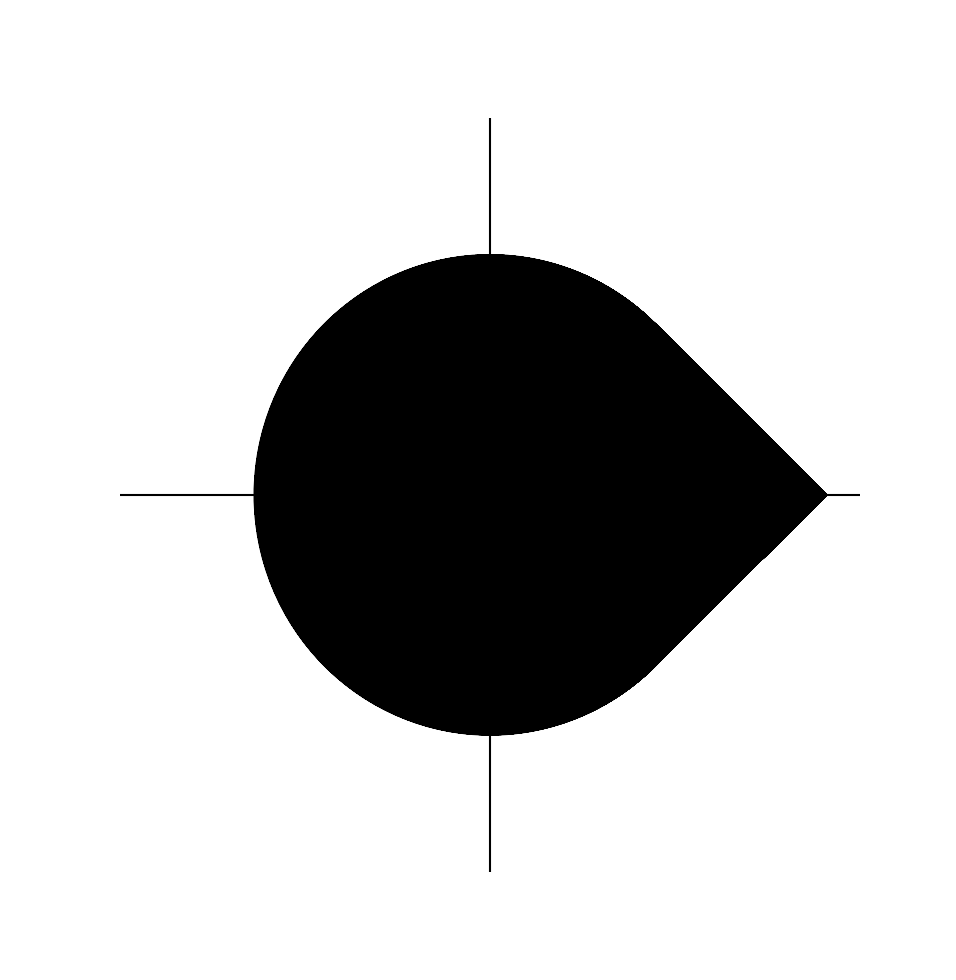
\includegraphics[width=0.5\textwidth]{approach-region-7}
\caption{A visualization of $\Omega_{\alpha}$, for a moderately large $\alpha$. Note that the only boundary point included in $\Omega_{\alpha}$ is $1$. }
\end{figure}
Let $0 < \alpha < 1$.
We refer to the open convex hull of
\[
	\{z \in \mathbb{C};\ |z| < \alpha\} \cup \{1\},
\]
that also includes $1$, as \emph{the nontangential approach region of $1$}, denoted by $\Omega_{\alpha}$.
We will also use the rotated version, $e^{i\theta}\Omega_{\alpha}$.
Let $u: \mathbb{D} \rightarrow \mathbb{C}$.
Its \emph{nontangential maximal function} is defined on $\mathbb{T}$ by
\[
	(N_{\alpha}u)(e^{it}) = \sup \{|u(z)|;\ z \in e^{it}\Omega_{\alpha}\}.
\]
We say that $u$ has \emph{nontangential limit $\lambda$ at $e^{it}$} if, for all $0 < \alpha < 1$,
\[
	\lim_{k \rightarrow \infty} u(z_k) = \lambda
\]
for all sequences $(z_k)_{k \in \mathbb{N}}$ in $e^{it}\Omega_{\alpha}$ that converge to $e^{it}$.
\end{definition}
\begin{lemma}
\label{FMRlemma2}
If $f$ is in $H^1$ then
\begin{enumerate}
\item \label{p1}
its nontangential limits, $F$, exist almost everywhere on $\mathbb{T}$,
\item \label{p2}
$F$ is in $L^1(\mathbb{T})$, and
\item \label{p3}
$f = P[F]$.
\end{enumerate}
\end{lemma}
\begin{proof}
Let $g$ and $h$ be functions in $H^2$ such that $f = g \cdot h$, as described above.
We have by Lemma \ref{FMRlemma3b} functions $G$ and $H$ in $L^2(\mathbb{T})$ such that $g = P[G]$ and $h = P[H]$.
Theorem $11.23$ in \citep{rudin2} (along with discussion on the prior page) states that if $h$ is in $L^1(\mathbb{T})$ then $P[h]$ has nontangential limit $h(e^{it})$ at almost every $e^{it}$.
We also have by the Hölder inequality that on a finite measure space (such as $\mathbb{T}$ with the Lebesgue measure) $\|h\|_1 \leq \|h\|_2$.
So $g$ and $h$ have nontangential limits almost everywere on $\mathbb{T}$.
This tells us that $f$ also has nontangential limits almost everywhere on $\mathbb{T}$, since $f = g \cdot h$.
By $f \leq h^2$ we have that $N_{\alpha}f \leq (N_{\alpha}h)^2$, and therefore $N_{\alpha}f \in L^1(\mathbb{T})$.
Let $F$ be the tangential limit of $f$.
We have that $|F| \leq N_{\alpha}f$ where $F$ is defined, so $F$ is also in $L^1(\mathbb{T})$.
Note that
\[
	\lim_{r \rightarrow 1} \|F - f_r\|_1 = \lim_{r \rightarrow 1} \int |F - f_r|\ d\sigma = 0
\]
since $f_r \rightarrow F$ holds almost everywhere and $|f_r| < N_{\alpha}f$ allows us to use dominated convergence.
We can also represent $f_r$ by its Poisson integral, for $r < 1$, that is
\[
	f_r(z) = \frac{1}{2\pi} \int_{-\pi}^{\pi} P(z, e^{it})f_r(e^{it})\ dt.
\]
Letting $r$ go to $1$ gives us
\[
	f(z) = \frac{1}{2\pi} \int_{-\pi}^{\pi} P(z, e^{it})F(e^{it})\ dt,
\]
namely, $f$ is the Poisson integral of $F$.
\end{proof}
\begin{theorem}[F. and M. Riesz theorem]
If $\mu$ is a complex Borel measure on $\mathbb{T}$ and
\[
	\int e^{-int}\ d\mu = 0
\]
for $n = -1, -2, ...$, then $\mu \lll \sigma$.
\end{theorem}
If we take a second look at the outline of proof given earlier we see that most of the work has been done.
All that's left is to show that the condition given in the theorem implies that $P[d\mu]$ is in $H^1$.
\begin{proof}
Let $f = P[d\mu]$.
If we set $z = re^{i\theta}$ we get that
\[
	P(z, e^{it})
		= P_r(\theta - t)
		= \sum_{n \in \mathbb{Z}} r^{|n|}e^{in(\theta - t)}
		= \sum_{n \in \mathbb{Z}} r^{|n|}e^{in\theta}e^{-int}.
\]
We can use the assumption of the theorem to write $f$ as a power series by
\begin{align*}
	f(z) 
	&= \int_{\mathbb{T}} P(z, e^{it})\ d\mu(e^{it}) \\
	&= \int_{\mathbb{T}} \sum_{n \in \mathbb{Z}} r^{|n|}e^{in\theta}e^{-int}\ d\mu(e^{it}) \\
	&= \sum_{n \in \mathbb{Z}} r^{|n|}e^{in\theta} \int_{\mathbb{T}} e^{-int}\ d\mu(e^{it}) \\
	&= \sum_{n = 0}^{\infty} r^n e^{in\theta} \int_{\mathbb{T}} e^{-int}\ d\mu(e^{it}) \\
	&= \sum_{n = 0}^{\infty} \hat{\mu}_n z^n,
\end{align*}
where $\hat{\mu}_n$ is the $n$-th Fourier coefficient of $\mu$.
This along with \ref{FMRlemma1} gives us that $f \in H^1$.
We can now define a $F \in L^1(\mathbb{T})$, by \ref{FMRlemma2} such that $f = P[F]$.
We have that
\[
	\int_{\mathbb{T}} P(z, e^{it})\ d\mu(e^{it})
	=
	\int_{-\pi}^{\pi} P(z, e^{it}) F(e^{it})\ d\sigma
\]
so it follows from \ref{FMRlemma3} that $d\mu = F\ d\sigma$, namely $\mu \lll \sigma$.
\end{proof}
\begin{corollary}
\label{fmrieszcor}
Every annihilating measures of $\mathcal{A}|_{\mathbb{T}}$ is absolutely continuous with regards to the Lebesgue-measure on $\mathbb{T}$.
\end{corollary}
\begin{proof}
Let $\mu$ be an annihilating measure of $\mathcal{A}|_{\mathbb{T}}$.
By definition we have that
\[
	\int f\ d\mu = 0
\]
for all $f \in \mathcal{A}|_{\mathbb{T}}$.
Now since $t \mapsto e^{-int}$ is entire for $n = -1, -2, ...$ we have that their restriction to $\mathbb{T}$ are in $\mathcal{A}|_{\mathbb{T}}$.
Thus,
\[
	\int e^{-int}\ d\mu = 0
\]
for all $n = -1, -2, ...$ and $\mu \lll m$.
\end{proof}



\section{Rudin-Carleson theorem}
\label{section2}
We will refer to the \emph{closed unit square} in $\mathbb{C}$ by
\[
	S = \{z;\ \max(|\Re z|, |\Im z|) \leq 1\}.
\]
The square with side-lengths $a$ and bottom-left corner at $w$ is then denoted by $w + aS$.

To adequately discuss the main result of this theorem we need a few fundamentals about closed set in $\mathbb{R}$ of Lebesgue-measure zero.
Let $K$ be such a set.
We can show by contradiction that $K$ is totally disconnected.
Recall that a set is totally disconnected if each connected component is a singleton.
If $K$ was not totally disconnected it would have an open subset meaning its measure could not be zero.
Another important thing to note is that $K$ could include an uncountable number of elements.
Results like \ref{mylemma} would be trivial if this were not the case.
A famous example of an uncountable, closed set of Lebesgue-measure zero is the Cantor set.
We will also make use of the following lemma:
\begin{lemma}
\label{somelemma}
Let
	$\varepsilon > 0$,
	$K$ be a closed subset of $]0, 1]$ of Lebesgue-measure zero,
	and $f: K \rightarrow \mathbb{C}$.
Then there exist pairwise disjoint $E_1, E_2, ..., E_n$ and $w_1, w_2, ..., w_n$ such that 
\[
	E_1 \cup E_2 \cup ... \cup E_n = K
\]
and
\[
	f(E_k) \subset w_k + \varepsilon S \tag*{$k = 1, 2, ..., n$.}
\]
\end{lemma}
\begin{proof}
It suffices to show that the image of each partition is contained in a circle with radius $\varepsilon$ since each square includes a circle.
Recall that a point $x$ in a set $A$ is a \emph{limit point of $A$} if it is in the closure of $A \setminus \{x\}$.
Since K is compact, f is uniformly continuous
This means we can set $\delta > 0$ such that $|f(x) - f(y)| < \varepsilon$ if $|x - y| < \delta$.
Let $a_1, a_2, ..., a_{p + 1}$ be a strictly increasing sequence in $]0, 1]$ such that $a_{k + 1} - a_k < \delta/2$, for $k = 1, 2, ..., p$ and $E_k = E \cap ]a_k, a_{k + 1}]$, for $k = 1, 2, ..., p$.
The only problem with this decomposition is that the sets may not be closed.
More concretely, if $a_k$ is a limit point of $E$ then $E_k$ may not be closed, for $k = 1, 2, ..., p$.
If we could replace $a_k$ by a point in $I = ]a_k, a_{k + 1}[$ that was not a limit point of $E$ then this problem will be solved.
Let's assume no such point exists and show it leads to a contradiction.
This implies that $E \cap I$ is dense in $I$, but this would imply that $E$ contains $I$, since $E$ is closed and therefore $E \cap I$ closed in $I$.
But $E$ can't contain an open set since $E$ is of Lebesgue-measure zero.
\end{proof}
We can show that \ref{somelemma} still holds if we replace $]0, 1]$ by $\mathbb{T}$ in the same way.
This is the context we will later use it in.

In the discussion before the proof of \ref{mylemma} a logarithm is used.
This is the base $2$ logarithm, specifically it satisfies $\log 2^x = x$.

\begin{theorem}[Rudin-Carleson theroem]
\label{rudincarleson}
Let $E$ be a closed subset of $\mathbb{T}$ of Lebesgue-measure $0$,
	let $f$ be a continuous function on $E$,
	and let $T$ be a subset of $\mathbb{C}$ homeomorphic to $\overline{\mathbb{D}}$ such that $f(\overline{\mathbb{D}}) \subset T$.
Then there exists an $F \in \mathcal{A}$, such that $F = f$ on $E$ and $F(\overline{\mathbb{D}}) \subset T$.
\end{theorem}
This will be proved as Rudin did in his original paper \citep{rudin}.
We will split up the proof into several lemmas.
The first few lemmas are dedicated to showing the result holds for continuous simple functions, and the last lemma bridges the gap.
\begin{lemma}
\label{mylemma}
Let $H$ be a closed set of Lebesgue-measure zero.
Then there exists a function $h: \mathbb{T} \rightarrow [1, \infty]$ such that 
\begin{enumerate}
\item
% COMMENT(gardar): er sigma Lebesgue málið?
$h$ is in $L^1(\mathbb{T}, m)$
\item
$h|_{\mathbb{T} \setminus H}$ is in $C^{\infty}$.
\item
$h(z) = \infty$ if and only if $z$ is in $H$.
\item
$\lim_{w \rightarrow z} h(w) = \infty$ for all $z$ in $H$.
\end{enumerate}
\end{lemma}
Recall from set theory that if $(X, d)$ is a metric space, $A$ is a subset of $X$ and $x$ is a point of $X$ then the distance between $x$ and $A$ is defined by
\[
	d(x, A) = \inf_{a \in A} d(x, a).
\]
Furthermore, if $A$ is closed then the infimum is obtained at some point in $A$, namely, there exists a point $y \in A$ such $d(x, y) = d(x, A)$.
Let $X = [0, 1]$ and $H$ be some closed set of Lebesgue-measure zero.
We will, for reasons that will be made clear later, assume that $\{0, 1\} \subset H$.
We can now define function $V_H: [0, 1] \rightarrow [0, 1]$ and $H_H: [0, 1] \rightarrow [0, 1]$ such that
\[
	d(x, H \cap [0, x]) = d(x, V_H(x))
	\quad \text{and} \quad
	d(x, H \cap [x, 1]) = d(x, H_H(x)).
\]
Intuitively, $H_H(x)$ is the point in $H$ that's to the right of $x$ and is closest to $x$ and $V_H(x)$ is the point in $H$ that's to the left of $x$ and is closest to $x$.
So all points $x$ in $[0, 1] \setminus H$ are on the open interval $]V_H(x), H_H(x)[$.
We will define function $f: [0, 1] \rightarrow [0, \infty]$ by
\[
	f_H(x) = 2\log \left ( \frac{H_H(x) - V_H(x)}{2} \right ) - \log((x - V_H(x))(H_H(x) - x))
\]
and show that this is the desired function.
\begin{figure}[h]
\centering
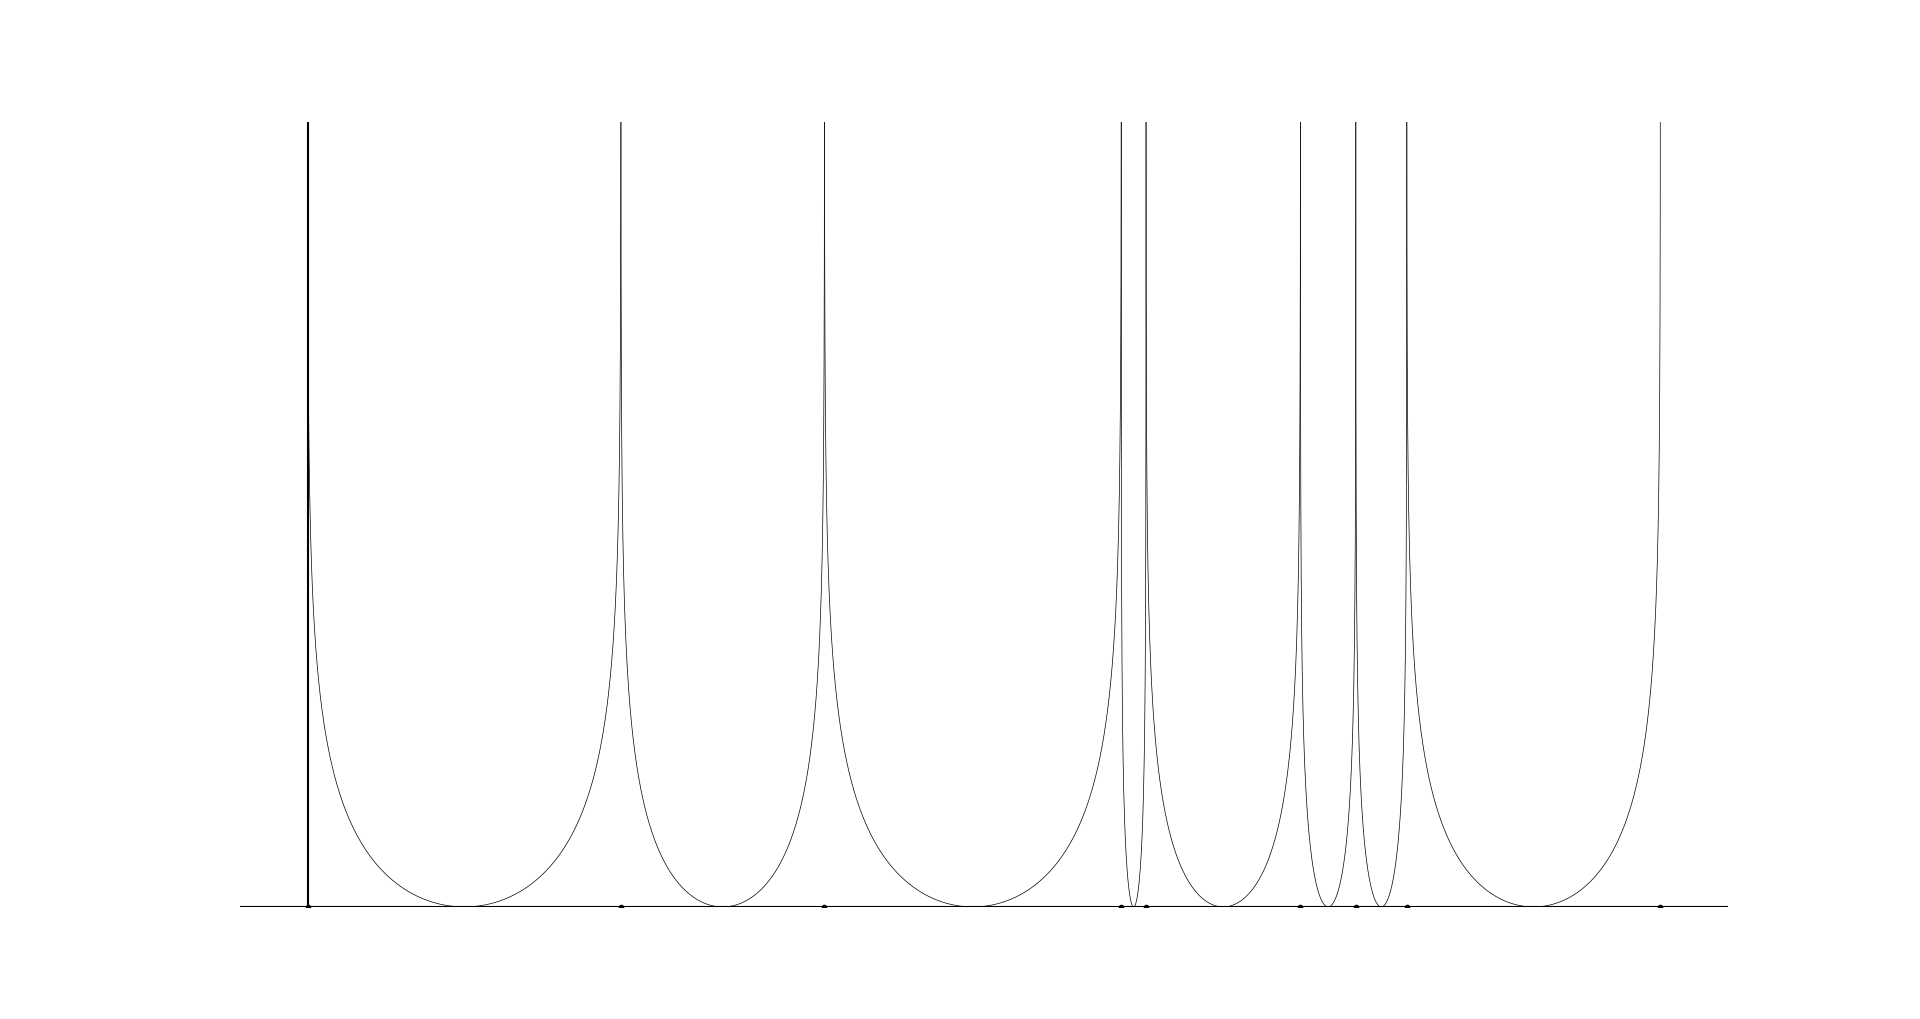
\includegraphics[width=1\textwidth]{graph8}
\caption{An example of $f_H$ where $H$ includes nine points. The points of $H$ are represented by circles. }
\end{figure}

Let's first define a family of functions indexed with $a, b \in \mathbb{R}$ by
\[
	f_{a, b}: [a, b] \rightarrow [0, \infty],
	x \mapsto 2\log \left ( \frac{b - a}{2} \right ) - \log((x - a)(b - x))
\]
and show they satisfy the following properties:
\begin{enumerate}
\item
$f_{a, b}(a + (b - a)2^{-n}) \leq n$,
\item
$f_{a, b}(x) = f_{a, b}(b + a - x)$.
\end{enumerate}
\begin{figure}[h]
\centering
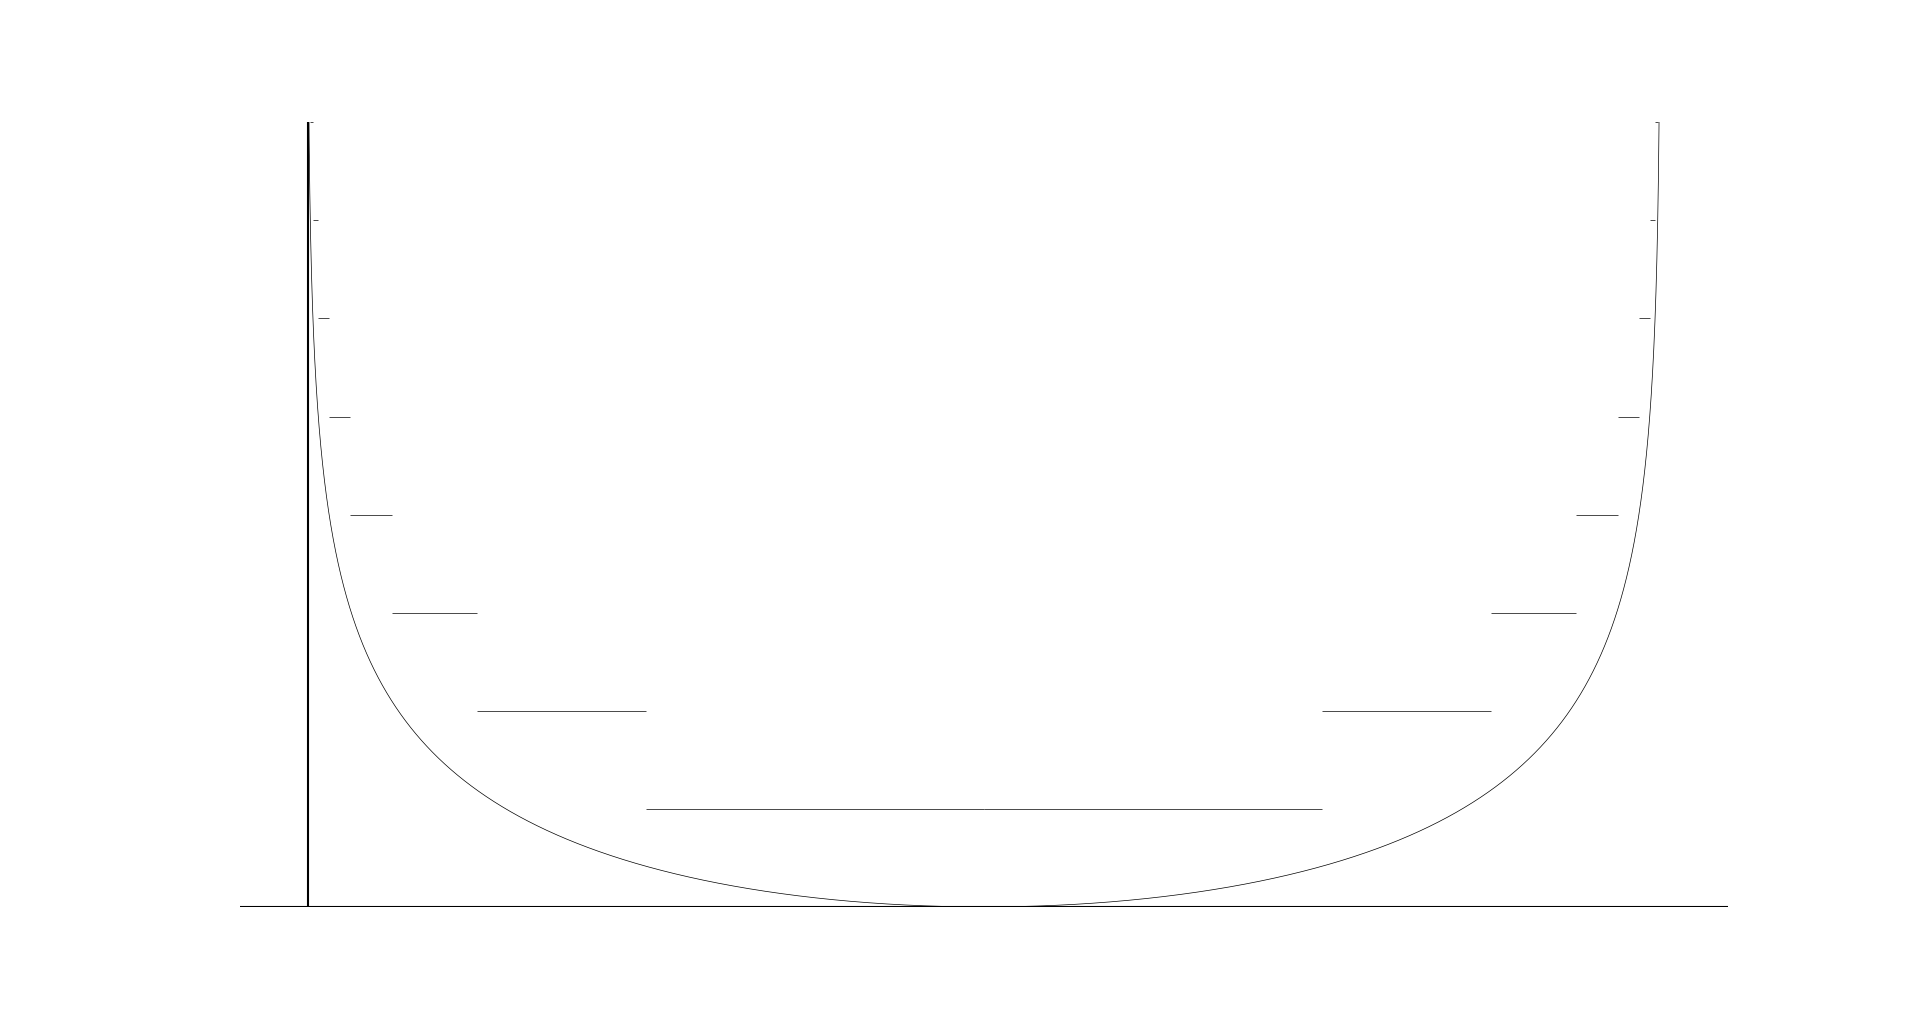
\includegraphics[width=1\textwidth]{graph2}
\caption{The graph of $f_{0, 1}$ and $g_{0, 1}$.}
\end{figure}
The first point gives us a handy estimate and the second tells us $f_{a, b}$ is symmetric around $(a + b)/2$.
We have that
\begin{align*}
	f_{a, b}(a + (b - a)2^{-n})
	&= 2\log (b - a) - 2\log 2 - \log (((b - a)2^{-n})(b - a - (b - a)2^{-n}))\\
	&= 2\log (b - a) - 2 - \log ((b - a)^2(1 - 2^{-n})2^{-n})\\
	&= 2\log (b - a) - 2 - 2\log (b - a) - \log (1 - 2^{-n}) - \log 2^{-n}\\
	&= n - (2 + \log (1 - 2^{-n}))\\
	&\leq n.
\end{align*}
To show the second property we consider the case where $a = -b$, that is we translate so that the midpoint between them is $0$.
Then
\begin{align*}
f_{-b, b}(-x)
&= 2 - \log ((-x + b)(b + x))\\
&= 2 - \log ((b - x)(x - (-b)))\\
&= f_{-b, b}(x).
\end{align*}
These two points together tell us that we can bound $f_{a, b}$ above by
\[
	g_{a, b}(x) =
	\left \{
	\begin{array}{l l}
	n, & \text{ if } 2^{-n} \leq \frac{x - a}{b} < 2^{-n + 1}\\
	g_{a, b}(a + b - x) , & \text{ if } \frac{x - a}{b} > \frac{1}{2}
	\end{array},
	\right .
\]
namely a function taking integer values.
It is more convenient to look at $g_{a, b}$ instead of $f_{a, b}$ because the former can trivially be shown to be the limit of a monotone sequence of simple functions.
Let's look at the case where $a = 0$ and $b = 1$.
Let $g = g_{0, 1}$ and
\[
	g_n(x) = \left \{
	\begin{array}{l l}
	g(x), & \text{ if } g(x) \leq n \\
	0, & \text{ else}.
	\end{array}
	\right .
\]
We can now integrate $g$ by
\begin{align*}
	\int g\ dm
	&= \int \lim_{n \rightarrow \infty} g_n\ dm\\
	&= \lim_{n \rightarrow \infty} \int g_n\ dm\\
	&= \lim_{n \rightarrow \infty} \sum_{k = 1}^n k2^{-k}\\
	&= \sum_{k \in \mathbb{N}} k2^{-k}\\
	&< \infty
\end{align*}
where the second equality is by monotone convergence and the last inequality is by the ratio test.
This rationale also holds for general $a$ and $b$, since $a$ does not effect the value of the integral and $b$ scales it.
We can, as a side note, compute the limit of this series by setting, for $x > 1$,
\[
	f(x) = \frac{2}{1 - x} = -2\sum_{n \in \mathbb{N}} x^{-k}
\]
and note that
\[
	f'(x) = 2\sum_{n \in \mathbb{N}} kx^{-k - 1},
\]
so the limit of the series is $f'(2)$.
We also have that
\[
	f'(x) = \frac{d}{dx}\frac{2}{1 - x} = \frac{2}{(1 - x)^2}
\]
so $f'(2)$, and therefore the limit of the series, is $2$.

Let's now go back to $f_H$.
Note that we can locally look at $f$ as a function in $\{f_{a, b}\}_{a, b \in [0, 1]}$, that is, $f(x) = f_{V_H(x), H_H(x)}(x)$.
We can define a function
\[
	g_H(x) = g_{V_H(x), H_H(x)}(x)
\]
and a sequence of functions
\[
	g_n(x) = \left \{
	\begin{array}{l l}
	g_H(x), & \text{ if } g(x) \leq n \\
	0, & \text{ else}.
	\end{array}
	\right .
\]
We have that $(g_n)_{n \in \mathbb{N}}$ is monotone with limit $g$, similar to before, and $f \leq g$.
Note that, independent of $H$, we have
\[
	m(f_H^{-1}(k)) = 2^{-k}
\]
so
\begin{align*}
\int f_H\ dm
&\leq \int g_H\ dm\\
&= \int \lim_{n \rightarrow \infty} g_n\ dm\\
&= \lim_{n \rightarrow \infty} \int g_n\ dm\\
&= \lim_{n \rightarrow \infty} \sum_{k = 1}^n k2^{-k}\\
&= \sum_{k \in \mathbb{N}} k2^{-k}\\
&< \infty
\end{align*}
\begin{center}
\end{center}
by the same reasoning as before.

\begin{figure}[h]
\centering
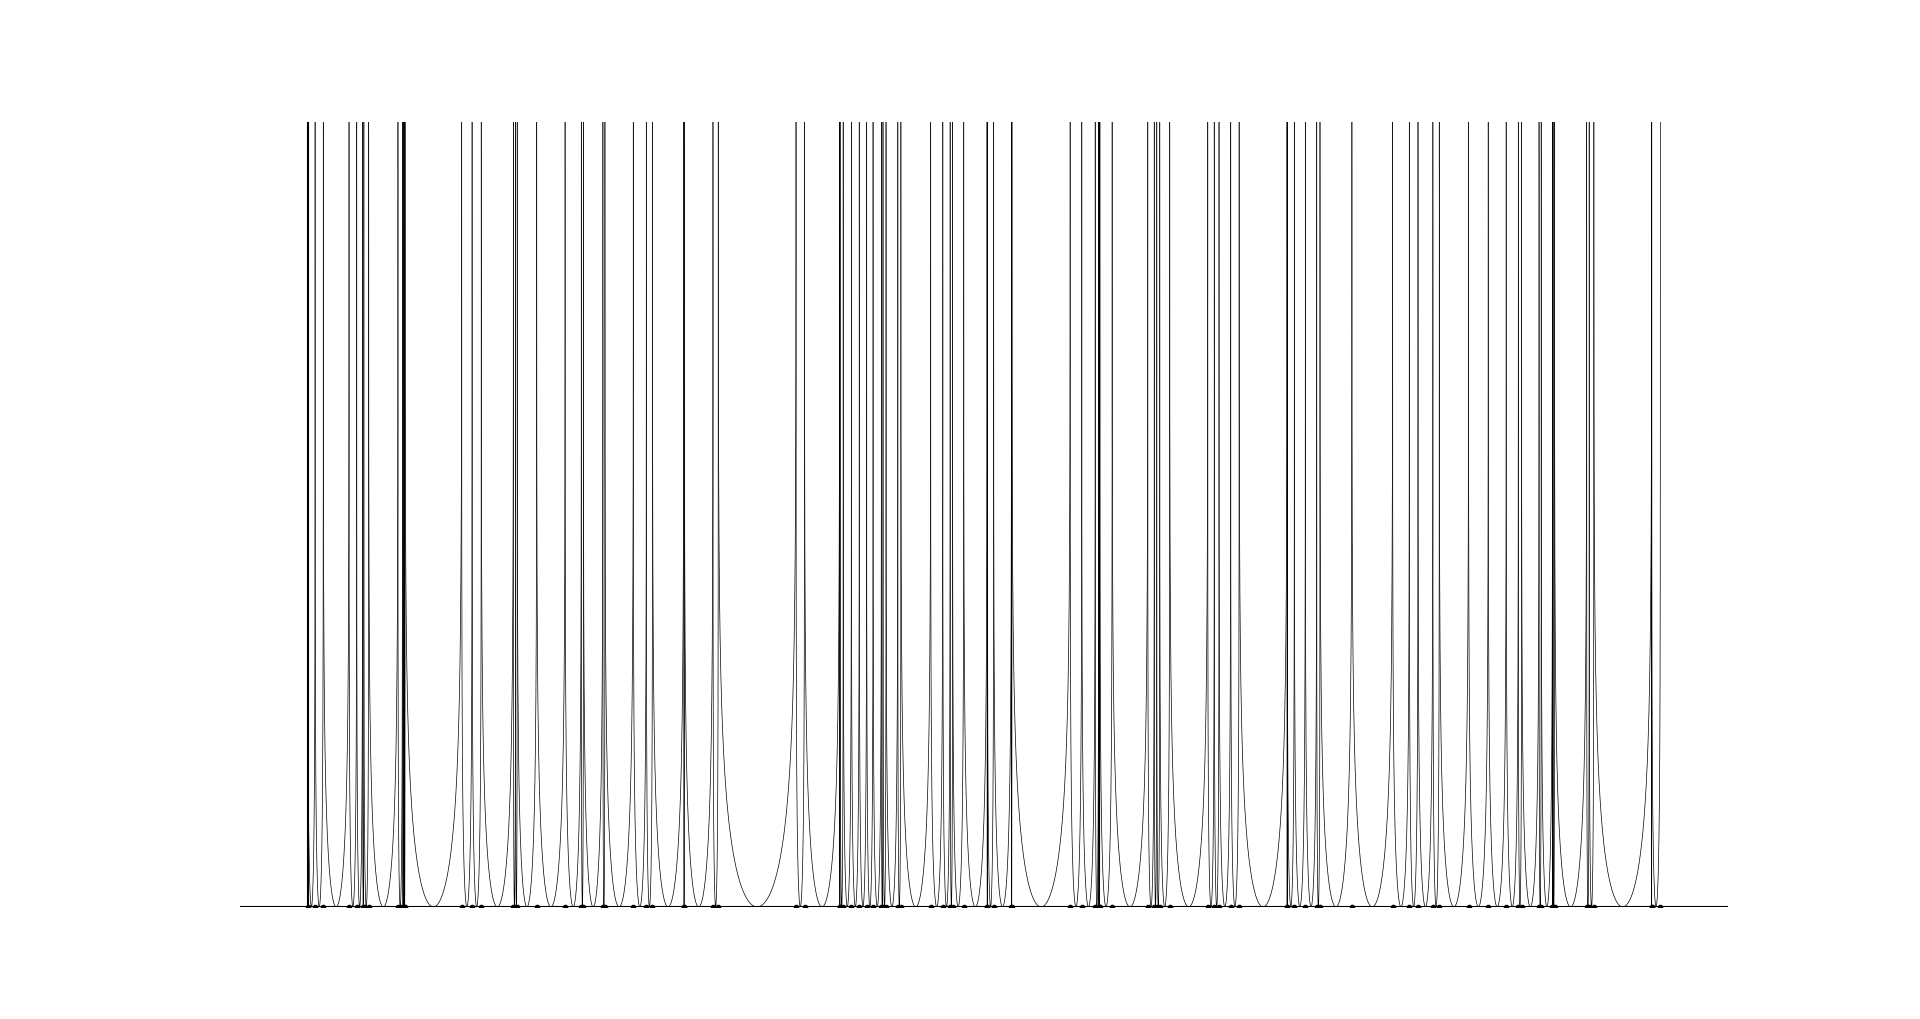
\includegraphics[width=1\textwidth]{graph101}
\caption{An example of $f_H$ where $H$ includes several points. The points of $H$ are represented by circles. }
\end{figure}
Note that we left some fundamentals unmentioned.
Specifically the fact that $f_H$ and $g_H$ are measurable.
To show that $g$ is measurable it suffices to show that $(g_n)_{n \in \mathbb{N}}$ are measurable.
We, therefore, can show that the preimage under $g_n$ of each point is measurable, since $g_n$ is simple for each $n$.
But the preimage is a (possibly uncountable) union of half-open intervals so it is the union of a closed set and an open set.
So $g$ is measurable.
To show that $f$ is measurable it suffices to show that $P_{\lambda} = \{x \in [0, 1];\ f(x) < \lambda\}$ is measurable for all $\lambda$ in $[0, \infty]$ \citep[lemma $1.3.9$]{tao}.
This trivially holds, since $P_{\lambda}$ is open.
\begin{proof}[Proof of \ref{mylemma}]
We may assume that $H$ is not empty, since the statement holds vacuously if that were the case.
We can also assume without loss of generality that $1$ is in $H$.
We can now use the injection $e^{it} \mapsto t/(2\pi)$, for $t \in [0, 2\pi[$,  to map $H$ to $H'$ a subset of $[0, 1]$ of measure zero.
We will add $1$ into $H$ to make sure it is closed.
The desired function is then $f_{H'}$ as desctibed above composed with the inverse of the prior injection with some constant added to make it strictly larger than $1$.
\end{proof}
\begin{lemma}
\label{rudinlemma1}
If $f$ is a simple continuous function on $E$ such that $\Re f \geq 0$, then there exists an $F \in \mathcal{A}$ such that $F = f$ on $E$ and $\Re F \geq 0$ on $\overline{\mathbb{D}}$.
\end{lemma}
\begin{proof}
It suffices to show that this holds if $f$ takes only two values on $E$, since simple functions are finite linear combinations of characteristic functions.
Let's assume these values are $0$ and $\alpha \neq 0$, with $\Re \alpha \geq 0$, $E_0 = f^{-1}(0)$, and $E_1 = f^{-1}(\alpha)$.
Our assumption that $f$ only takes two values then implies that $E_0 \cup E_1 = E$.

Let $u_H(z)$ be the Poisson integral of the function from \ref{mylemma}.
This function is continuous on $\mathbb{T} \setminus H$, $u_H|_H = \infty$, and $\lim_{z \rightarrow w} u_H(z) = \infty$ for $w \in H$ \citep[page $234$]{rudin2}.
Let's set $v_H$ as the conjugate harmonic of $u_H$ and define
\[
	g_H(z) =
	\left \{
		\begin{array}{l l}
		u_H(z) + iv_H(z), & z \in \mathbb{D} \setminus H\\
		\infty, & \text{otherwise}
		\end{array}.
	\right .
\]
By our construction of $u_H$ we see the $\Re g_H > 1$, so it has a well defined square root.
Let's call it $h_H$ and define
\[
	q = \frac{h_{E_1}}{h_{E_0} + h_{E_1}}.
\]
Note that $|\arg h_H(z)| \leq \pi/4$ since if a $w \in \mathbb{C}$ had an argument outside of this range then its square would have and argument outside of the range $[-\pi/2, \pi/2]$ meaning $\Re w^2 < 0$.
Also, $q(z) = 0$ if and only if $h_{E_0} = \infty$, so $q$ is zero only on $E_0$, and $q(z) = 1$ if and only if $h_{E_1} = \infty$, so $q$ is one only on $E_1$.
We now want to show that $0 \leq \Re q \leq 1$.
We will let $z, w \in \mathbb{C}$, with $|\arg z|, |\arg w| < \pi/4$ and $\Re z, \Re w > 1$, and show that $0 < \Re z/(w + z) < 1$.

Note first that
\[
	\frac{z}{w + z}
	=
	\frac{1}{w/z + 1}
\]
so 
\[
	\arg \frac{z}{w + z} = -\arg \left ( \frac{w}{z} + 1 \right )
\]
and
\[
	|\arg w/z| = |\arg w - \arg z| \leq |\arg w| + |\arg z| < \pi/4 + \pi/4 = \pi/2.
\]
So $w/z$ is in the right halfplane and, therefore $w/z + 1$ is as well.
We have now shown that $0 < \Re z/(w + z)$.
Note that $0 < \Re z/(w + z) \implies 0 > \Re -w/(w + z)$ due to $z$ and $w$ being constrained in the same manner, and
\begin{align*}
	0
	&> \Re \frac{-w}{w + z}\\
	&= \Re \frac{z - (z + w)}{w + z}\\
	&= \Re \left ( \frac{z}{w + z} - 1 \right )\\
	&= \Re \frac{z}{w + z} - 1\\
	\implies 1 &> \Re \frac{z}{z + w}.
\end{align*}
So we have shown that
\[
	0 < \Re \frac{z}{z + w} < 1.
\]

We have now constructed a function $q$ that maps $\overline{\mathbb{D}}$ to the ribbon $\{z;\ 0 \leq \Re z \leq 1\}$.
We then let $\Phi$ be the conformal mapping from the ribbon $\{z;\ 0 \leq \Re z \leq 1\}$ to $\{z;\ 0 \leq \Re z \leq \Re \alpha\}$.
We will also choose $\Phi$ such that $\Phi(0) = 0$ and $\Phi(1) = \alpha$.
We can then let $F = \Phi \circ q$ and conclude the proof.

\end{proof}
\begin{lemma}
\label{rudinlemma2}
If $f$ is a simple continuous function on $E$ that maps $E$ into $T \subset \mathbb{C}$ homeomorphic to $\overline{\mathbb{D}}$, then there exists a function $F \in \mathcal{A}$, such that $F = f$ on $E$ and $F$ maps $\overline{\mathbb{D}}$ into $T$.
\end{lemma}
\begin{proof}
Let $z_0 \in T \setminus f(E)$ and $\Phi$ be a conformal mapping from the right halfplane to the interior of $T$ such that $\Phi(\infty) = z_0$.
There exists a $g \in \mathcal{A}$ that extends $\Phi^{-1} \circ f$, according to Lemma \ref{rudinlemma1}.
The desired function in then obtained with $F = \Phi \circ g$.
\end{proof}
\begin{lemma}
\label{rudinlemma3}
If $f$ is a continuous function on $E$ which maps $E$ into $S$ then there exists a sequence $(f_n)_{n \in \mathbb{N}}$ of simple continuous function on $E$ such that
\[
	f(x) = \sum_{n \in \mathbb{N}} f_n(z)
	\text{ and }
	f_n(E) \subset 2^{-n}S.
\]
\end{lemma}
\begin{proof}
We will set $f_0 = 0$ and construct $f_n$ iteratively.
Assuming $f_0, f_1, ..., f_{n - 1}$ have been constructed such that
\[
	\lambda_{n - 1}(E) \subset 2^{1 - n}S
\]
with $\lambda_{n - 1} = f - \sum_{k = 0}^{n - 1}f_k$.
According to \ref{somelemma} we have can write $E$ as the union of disjoint closed sets $E_1, E_2, ..., E_p$ such that the oscillation of $\lambda_{n - 1}$ is less than $2^{-n}$ on each $E_k$.
So we can define $Q_k \subset 2^{1 - n}S$ for $k = 1, 2, ..., p$ such that $Q_k = 2^{-n}S + a_k$ for some $a_k \in S$.
We can choose $c_k \in Q_k \cap 2^{-n}S$ since $Q_k$ has side length $2^{-n}$ and is a subset of $2^{-n + 1}$ and both are closed.
We can now define
\[
	f_n(z) = c_k, \tag*{$z \in E_k,\ k = 1, 2, ..., p$.}
\]
If we then look at $\lambda_n = f - \sum_{k = 0}^nf_k = \lambda_{n - 1} - f_n$ we see that $\lambda_n(E) \subset 2^{-n}S$ due to the way we decomposed $E$ into $E_1, E_2, ..., E_p$ using the oscillations of $\lambda_{n - 1}$.
This means we can continue the process.
\end{proof}
\begin{proof}[Proof of \ref{rudincarleson}]
Let's first show the result for $T = S$.

Let $f_n$ be the functions from Lemma \ref{rudinlemma3}.
According to Lemma \ref{rudinlemma2} we have functions $g_n \in \mathcal{A}$ which extend $f_n$ and map $\overline{\mathbb{D}}$ into $2^{-n}S$.
We then define
\[
	F = \sum_{n \in \mathbb{N}} g_n
\]
on $\overline{\mathbb{D}}$.
To show that $F$ is in $\mathcal{A}$ it suffices to show that series converges uniformly.
Let $M_n = 2^{-n + 1}$ and note that $|g_n(z)| \leq \sqrt{2}\cdot 2^{-n} < 2^{-n + 1} = M_n$ and
\[
	\sum_{n \in \mathbb{N}} M_n
	=
	\sqrt{2}\sum_{n \in \mathbb{N}} 2^{-n} =
	\sqrt{2} < \infty
\]
so the Weierstrass M-test tells us that $F$ converges uniformly.
We also have that
\[
	\Re F = \sum_{n \in \mathbb{N}} \Re g_n \leq \sum_{n \in \mathbb{N}} 2^{-n} = 1.
\]
It can be shown in the same manner that $\Im F \leq 1$, so $F$ maps into $S$.
Lastly, for $z \in E$ we have that
\[
	F(z) = \sum_{n \in \mathbb{N}} g_n(z) = \sum_{n \in \mathbb{N}} f_n(z) = f(z)
\]
so $F$ is an extension of $f$.

To prove the result for a general $T$ we first let $\Phi: T \rightarrow S$ be the map provided to us by \ref{contrmt}.
We will also let $g = f \circ \Phi$.
Note that it maps $E$ into $S$, so we can use what we showed above to find $G \in \mathcal{A}$ that extends $g$ and maps into $S$.
We finally set $F = G \circ \Phi^{-1}$.
On $E$ we have that
\[
	F = G \circ \Phi^{-1} = g \circ \Phi^{-1} = f \circ \Phi \circ \Phi^{-1} = f,
\]
so $F$ extends $f$.
It is also a composition of functions in $\mathcal{A}$ so it is also in $\mathcal{A}$.
\end{proof}



\section{A generalization of the Rudin-Carleson theorem}
\label{section3}
An obvious next step would be a Rudin-Carleson theorem in several complex variables.
It is tempting to keep the constraints on $E$ unchanged, namely that it is of Lebesgue-measure zero, but this won't work.
Take as an example $f: E \rightarrow \mathbb{C}$ with $E = \mathbb{T} \times \{0\}$ and $f(z, w) = \overline{z}$.
Clearly $E$ is of Lebesgue-measure but $f$ cannot be extended.
If we assume it could be extended to some $g = (g_1, g_2)$ in $\mathcal{A}^2$ then, by definition, $g_1$ would be holomorphic on $\mathbb{D}$ and continuous $\overline{\mathbb{D}}$.
Its holomorphicity tells us that its integral over the boundary of $r\mathbb{T}$ for $0 < r < 1$ is zero.
But on $\mathbb{T}$ we have that $g(z) = \overline{z}$ so its integral over $\mathbb{T}$ is not zero.
That is, we have that
\[
	\lim_{r \rightarrow 1} \int_{r\mathbb{T}} g_1(z)\ dz \neq \int_{\mathbb{T}} g_1(z)\ dz
\]
so $g_1$ is not continuous.

There is however a theorem of Bishop that gives a sufficient condition on $E$ \citep{bishop}.
% COMMENT(gardar): banger alert
\begin{theorem}[Bishop's general Rudin-Carleson theorem]
\label{bishopstheorem}
Let $X$ be a compact Hausdorff space,
	$V = (C(X), \| \cdot \|_{\infty})$,
	$B$ be a closed subspace of $C(X)$,
	$B^{\bot}$ be the annihilating measures of $B$,
	$S$ be a closed subset of $X$ that is $\mu$-null for all $\mu \in B^{\bot}$, % TODO kannski breyta í E
	$f$ be a continuous function on $S$,
	and continuous $\Xi: X \rightarrow [0, \infty[$ such that $|f| < \Xi$ on $S$.
Then there exists a $F \in B$ such that $F = f$ on $S$ and $|F| < \Xi$ on $X$.
\end{theorem}
The following lemma makes the proof simple.
The proof of the lemma is sort of split in two.
The earlier part is to show that $f$ is in the closure of the image of the restriction mapping and the latter part shows that leads the existence of $F$.
\begin{lemma}
\label{bishoplemma}
Assume $|f| < r < 1$ on $S$.
Then there exists a $F \in B$ such that $F = f$ on $S$ and $\|F\| < 1$.
\end{lemma}
\begin{proof}
Let $U_r$ be the subset of $B$ defined by $U_r = \{g;\ \|g\| < r\}$ and $\phi$ be the mapping from $B$ to $C(S)$ that sends a member of $B$ to its restriction on $S$.
It suffices to show that $f \in \phi(U_r)$.
Let's first show that $f$ is in $V_r = \overline{\phi(U_r)}$, by assuming otherwise, and showing it leads to a contradiction.
Note that if $f, g \in U_r$ and $t \in [0, 1]$ then
\[
	\|tf + (1 - t)g\| \leq t\|f\| + (1 - t)\|g\| \leq tr + (1 - t)r = r
\]
so $tf + (1 - t)g$ is also in $U_r$, showing it is convex.
Its closure, $V_r$, is then convex as well.

We can, by Hahn-Banach, define a bounded linear functional $\alpha$, such that $\alpha(f) > 1$ and $|\alpha| < 1$, on $V_r$.
We can then define a measure $\mu_1$ by the Riesz representation theorem that satisfies
\[
	\alpha(g) = \int g\ d\mu_1
\]
for all $g \in C(S)$.
We will refer to the associated functional on $B$ by $\beta(g) = \alpha(\phi(g))$.
Since $\phi(g) \in V_r$ for all $g \in U_r$ we have that
\[
	|\beta(g)| = |\alpha(\phi(g))| < 1,
\]
for all $g \in U_r$,
	due to the construction of $\alpha$.
From this we get
\begin{align*}
	\| \beta \|
	&= \sup \{ |\beta(g)|;\ \|g\| < 1 \}\\
	&= \sup \{ (1/r)|\beta(g)|;\ \|g\| < r \}\\
	&\leq 1/r.
\end{align*}
Let's
	denote the Riesz representation of $\beta$ by $\mu_2$,
	set $\mu = \mu_1 - \mu_2$,
	and note that $\mu \in B^{\bot}$.
But
\[
	0 = \left | \int_S f\ d\mu \right | 
		\geq \int_S f\ d\mu_1 - r\|\mu_2\| 
		\geq \int_S f\ d\mu_1 - r\frac{1}{r}
		> 1 - r \frac{1}{r} = 0.
\]
This contradiction gives that $f \in V_r$.
We can now take a $F_1$ in $U_r$, and therefore also in $B$ such that $|f - F_1| < \lambda/2$ on $S$, with $\lambda := 1 - r$.
Remember that $F_1 \in U_r$ implies that $\|F_1\| < r$.
Now let $f_1 = f - F_1$ and use the same method as above to obtain an $F_2$ such that $\|F_2\| < \lambda/2$ and $|f - F_2| < \lambda/4$ on $S$.
Iterating this process yields a sequence $(F_n)_{n \in \mathbb{N}}$ from $B$ such that $\|F_n\| < 2^{1 - n}\lambda$ for $n > 1$ and
\[
	\left | f - \sum_{k = 1}^n F_k \right | < 2^{-n}\lambda
\]
on $S$ for $n > 1$.
We finally let 
\[
F = \sum_{k = 1}^{\infty} F_k.
\]
Now $F \in B$,
\[
	\|F\| \leq \|F_1\| + \|F - F_1\| \leq r + \sum_{k = 2}^{\infty}2^{1 - n}\lambda = r + \lambda = 1,
\]
and $F = f$ on $S$.
\end{proof}
\begin{proof}[Proof of \ref{bishopstheorem}]
Let $B_0$ be the closed subspace of $C(X)$ consisting of function $g$ such that $\Xi \cdot g \in B$.
We have that $B_0^{\bot} = B^{\bot}$, since $\Xi > 0$.
So we can use Lemma \ref{bishoplemma} for $B_0$ instead of $B$ and $f/\Xi$ instead of $f$.
This gives us a function $F_0 \in B_0$ such that $\Xi \cdot F_0 = f$ on $S$ and $\|F_0\| < 1$.
We set $F = \Xi \cdot F_0$ which is in $B$ by the construction of $B_0$.
Also note that $|F| < \Xi$ on $X$ and 
\[
	F = \Xi \cdot F_0 = \Xi \cdot f/\Xi = f
\]
on $S$.
\end{proof}
\begin{proof}[Alternative proof of \ref{rudincarleson}]
Let
	$X = \mathbb{T}$,
	$B = \mathcal{A}|_{\mathbb{T}}$,
	and $S$ be a closed set of Lebesgue-measure zero. 
Then, according to \ref{fmrieszcor}, $S$ is also a $B^{\bot}$-null.
So all requirements of \ref{bishopstheorem} are met.
\end{proof}

\appendix
\renewcommand{\chaptername}{Appendix}
\chapter{Applications of the general Rudin-Carleson theorem}
\label{section4}
\section{Classification of compact subsets of $\mathbb{C}$} 
Bishop's theorem can be seen as a classification of sets.
With this in mind, and looking at the case where $X = \mathbb{T}^n$ and $B = \mathcal{A}^n|_{\mathbb{T}}$, we have the following definition.
\begin{definition}
\label{bigdef}
Let $K$ be a closed subset of $\mathbb{T}^n = \{z \in \mathbb{C}^n;\ |z| = 1\}$.
We then say $K$ is a
\begin{enumerate}
	\item \emph{zero set} if there exists a function in $f \in \mathcal{A}^n$ such that $K = f^{-1}(0)$.
	\item \emph{peak set} if there exists a function in $f \in \mathcal{A}^n$ such that $K = f^{-1}(1)$ and $|f(z)| < 1$ for $z \in \overline{\mathbb{D}}^n \setminus K$.
	\item \emph{interpolation set} if every continuous function on $K$ extends via $\mathcal{A}^n$. 
	\item \emph{peak-interpolation set} if every non-zero continuous function $f$ on $K$ extends to $F \in \mathcal{A}^n$ such that $|F(z)| < \|f\|$ for $z \in \overline{\mathbb{D}}^n \setminus K$.
	\item \emph{null set} if $K$ has measure zero with regards to all annihilating measures of $\mathcal{A}^n$.
	\item \emph{totally null} if $K$ has measure zero with regards to all measure $\mu$ such that
			\[
				f(0) = \int_{\mathbb{D}} f\ d\mu
			\]
			for all $f \in \mathcal{A}^n$.
\end{enumerate}
\end{definition}
\begin{theorem}
	\label{bigtheorem}
	The six classes of sets described in \ref{bigdef} are equivalent.
\end{theorem}
The first few sections of chapter $10$ in \citep{rudin3} are dedicated to proving this large theorem.
One implication, namely that all null sets are peak-interpolation sets, follows directly from \ref{bishopstheorem}.

\section{A variation of Bishop's theorem}
Theorem \ref{bigtheorem} implies that the condition on $S$ in Bishop's theorem can't, generally, be relaxed.
If we fix a continuous $f: S \rightarrow \mathbb{C}$ we might, however, be a able to chose a different classification on $S$.
It seems at first, when looking at the proof of Bishop's theorem, that $S$ being $B^{\bot}$-null is only used to show that
\[
	\int_S f\ d\mu = 0.
\]
If this were the case, we restate the theorem for a continuous function $f: S \rightarrow \mathbb{C}$ and set $S$ such that the above equation holds.
This, however, leads to problems.

Let
	$S = E \cup F$ where $F$ is a closed subarc of $\mathbb{T}$ of non-zero Lebesgue-measure and $E$ is a singleton in $\mathbb{T} \setminus F$
	and let $f: S \rightarrow \mathbb{C}$ such that $f = 0$ on $F$ and $f \neq 0$ on $E$.
Then we have by \ref{fmrieszcor} that $E$ is $B^{\bot}$-null, so
\[
	\int_S f\ d\mu = \int_F f\ d\mu = 0.
\]
So let's assume $f$ can be extended to $F$ via $\mathcal{A}$.
We also know that $F$ is in $H^1$ because it's a continuous function on a compact set and we know that $f = 0$ must hold on $\mathbb{D}$
\citep[Theorem $13.4.11$]{greenkrantz}.
So $F$ is $0$ Lebesgue-almost everywhere and continuous, and therefore $0$ everywhere.
This is a contradiction, because $F = f$ on $\mathbb{T}$ and $f$ is not zero on $E$.

Looking further at the proof shows that the iteration in the second half doesn't work with $f$, since 
\[
	\int_S (f - F)\ d\mu = -\int_S F\ d\mu = 0
\]
doesn't have to hold for every $F$ in $\mathcal{A}|_{\mathbb{T}}$.

So $S$ would have to both satisfy
\[
	\int_S f\ d\mu = 0
\]
for all $\mu$ in $B^{\bot}$ and
\[
	\int_S F\ d\mu = 0
\]
for all $F$ in $B$ and $\mu$ in $B^{\bot}$.
This justifies the following alteration of Bishop's theorem.
\begin{theorem}[An alteration of the Bishop's general Rudin-Carleson theorem]
\label{bishopstheorem}
Let $X$ be a compact Hausdorff space,
	$V = (C(X), \| \cdot \|_{\infty})$,
	$B$ be a closed subspace of $C(X)$,
	$B^{\bot}$ be the annihilating measures of $B$,
	$S$ be a closed subset of $X$,
	$f$ be a continuous function on $S$,
	and continuous $\Xi: X \rightarrow [0, \infty[$ such that $|f| < \Xi$ on $S$.
If
\[
	\int_S f\ d\mu = 0
\]
for all $\mu$ in $B^{\bot}$ and
\[
	\int_S F\ d\mu = 0
\]
holds for all $F$ in $B$ and $\mu$ in $B^{\bot}$ then there exists a $F \in B$ such that $F = f$ on $S$ and $|F| < \Xi$ on $X$.
\end{theorem}


\bibliography{refs}

\end{document}
